% !TEX root = free221.tex

\chapter{Derivatives (2)}




\begin{quote}\itshape
    ``Leibniz never thought of the derivative as a limit''\\[1ex]
  \footnotesize~\hfill
  \href{http://www-history.mcs.st-and.ac.uk/Biographies/Leibniz.html}
  {www-history.mcs.st-and.ac.uk/Biographies/Leibniz.html}\\
\end{quote}




\medskip




\noindent
In Chapter~\ref{ch:derivs1} we saw two mathematical problems which led
to expressions of the form $\frac00$.  Now that we know how to handle
limits, we can state the definition of the derivative of a function.
\marginpar{\footnotesize\sffamily%
  
    \begin{picture} (72.000000,97.666667)(0,0)
    \put(0.0, 0.0){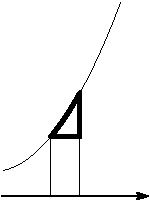
\includegraphics{04derivative-notation-ax.pdf}}
        \put( 24.33,  -4.67){\sffamily\itshape \makebox[0pt][c]{$a$}}
    \put( 36.33,  -4.67){\sffamily\itshape \makebox[0pt][l]{$x$}}
    \put( 40.33,  29.80){\sffamily\itshape \makebox[0pt][l]{$f(a)$}}
    \put( 40.33,  50.80){\sffamily\itshape \makebox[0pt][l]{$f(x)$}}
\end{picture}
\\
  
    \begin{picture} (72.000000,97.666667)(0,0)
    \put(0.0, 0.0){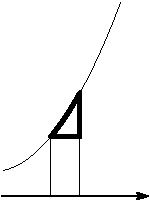
\includegraphics{04derivative-notation-ah.pdf}}
        \put( 24.33,  -4.67){\sffamily\itshape \makebox[0pt][c]{$a$}}
    \put( 36.33,  -4.67){\sffamily\itshape \makebox[0pt][l]{$a+h$}}
    \put( 40.33,  29.80){\sffamily\itshape \makebox[0pt][l]{$f(a)$}}
    \put( 40.33,  50.80){\sffamily\itshape \makebox[0pt][l]{$f(a+h)$}}
\end{picture}
\\
  
    \begin{picture} (72.000000,97.666667)(0,0)
    \put(0.0, 0.0){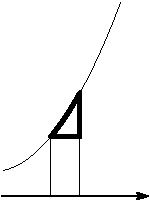
\includegraphics{04derivative-notation-xh.pdf}}
        \put( 24.33,  -4.67){\sffamily\itshape \makebox[0pt][c]{$x$}}
    \put( 36.33,  -4.67){\sffamily\itshape \makebox[0pt][l]{$x+h$}}
    \put( 40.33,  29.80){\sffamily\itshape \makebox[0pt][l]{$f(x)$}}
    \put( 40.33,  50.80){\sffamily\itshape \makebox[0pt][l]{$f(x+h)$}}
\end{picture}
\\
  
    \begin{picture} (72.000000,97.666667)(0,0)
    \put(0.0, 0.0){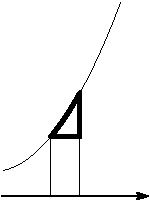
\includegraphics{04derivative-notation-xDx.pdf}}
        \put( 24.33,  -4.67){\sffamily\itshape \makebox[0pt][c]{$x$}}
    \put( 36.33,  -4.67){\sffamily\itshape \makebox[0pt][l]{$x+\Delta x$}}
    \put( 40.33,  29.80){\sffamily\itshape \makebox[0pt][l]{$f(x)$}}
    \put( 40.33,  50.80){\sffamily\itshape \makebox[0pt][l]{$f(x+\Delta x)$}}
\end{picture}
 }%
After computing a few derivatives using the definition we will spend
most of this section developing the \textit{differential calculus,}
which is a collection of rules that allow us to compute derivatives
without always having to use the basic definition.




\section{Derivatives Defined} 
%
\subsection{Definition} 
\label{def:derivative}\itshape
Let $f(x)$ be a function that is defined on an interval $(c, d)$
and let $a$ be a number in this interval.




We say that $f(x)$ is \emph{differentiable at $a$} if the limit
\begin{equation}\label{eq:derivative-defined}
  \lim_{x\to a} \frac{f(x)-f(a)}{x-a}
\end{equation}
exists, and (if it exists) we call the value of the limit the \emph{derivative
of the function $f$ at $a$}, and denote it as $f'(a)$.




\noindent
$f$ is called \emph{differentiable on the interval $(c, d)$} if it is
differentiable at every point $a$ in $(c,d)$.




\upshape




\subsection{Other notations}\label{sec:other-notations} 
We can substitute $x=a+h$ in the limit \eqref{eq:derivative-defined}
and let $h\to0$ instead of $x\to a$.  This gives the formula
\begin{equation}\label{eq:derivative-defined-a-plus-h}
  f'(a) = \lim_{h\to 0} \frac{f(a+h)-f(a)}{h},
\end{equation}
Often this equation is written with $x$ instead of $a$,
\begin{equation}\label{eq:derivative-defined-x-plus-h}
  f'(x) = \lim_{h\to 0} \frac{f(x+h)-f(x)}{h},
\end{equation}
and $\Delta x$ instead of $h$, which makes it look like this:
\begin{equation}\label{eq:derivative-defined-x-plus-Dx}
f'(x) = \lim_{\Delta x\to0} \frac{f(x+\Delta x) - f(x)}{\Delta x}.
\end{equation}
The interpretation is the same as in equation \eqref{eq:difference-quotient}
from \S~\ref{sec:rates-of-change} in Chapter II.  The numerator $f(x+\Delta x) -
f(x)$ represents the amount by which the function value of $f$ changes if we
increase its argument $x$ by a (small) amount $\Delta x$.  If we write $y=f(x)$
then we can call the increase in $f$
\[
\Delta y = f(x+\Delta x) - f(x),
\]
so that the derivative $f'(x)$ is
\[
f'(x) = \lim_{\Delta x\to0}\frac{\Delta y}{\Delta x}.
\]
\textsc{Gottfried Wilhelm von Leibniz}, one of the inventors of calculus,
came up with the idea that one should write this limit as
\[
\frac{dy}{dx}= \lim_{\Delta x\to0}\frac{\Delta y}{\Delta x},
\]
the idea being that after letting $\Delta x$ go to zero it didn't vanish,
but instead became an ``infinitely small quantity'', which Leibniz called
``$dx$''.  The result of increasing $x$ by this ``infinitely small quantity''
$dx$ is that $y=f(x)$ increases by another infinitely small quantity $dy$.
The ratio of these two infinitely small quantities is what we call the
derivative of $y=f(x)$.
\marginpar{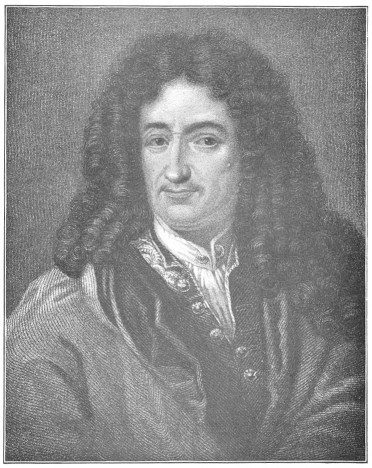
\includegraphics[width=90pt]{Wag_gottfried_wilhelm_leibnitz.jpg}\\
\centering\footnotesize\sffamily%
Leibniz (1646--1716)}




We began the semester by agreeing that there are no ``infinitely small
numbers'', and this makes Leibniz's notation difficult to justify.  In
spite of this we will often use his notation because it shortens
many formulas for derivatives, and it often makes intuitive sense.%
\footnote{So many people use Leibniz' notation that mathematicians have
  tried hard to create a consistent theory of ``infinitesimals'' that
  would allow you to compute with ``$dx$ and $dy$'' as Leibniz and his
  contemporaries would have done.  In the mid 20th century such a
  theory was finally created, and dubbed ``non-standard analysis.'' We
  won't mention it any further, but, as pointed out in a footnote in
  Chapter I, Keisler's calculus text using infinitesimals at\\
  \centerline{\url{http://www.math.wisc.edu/~keisler/calc.html}}\\
  is aimed at undergraduates, so you could have a look if you're
  interested.}


If $f(x)$ is a complicated function, we will often use ``operator notation'' for
the derivative $\dfrac{df}{dx}$, by writing it as
\[
  \frac{d}{dx}\left[f\right].
\]
The symbol $\frac{d}{dx}$ is shorthand for ``take the derivative of what
follows with respect to the variable $x$''.




\section{Direct computation of derivatives} 
\label{sec:direct-derivative-computation}




\subsection{Example -- The derivative of $f(x)= x^2$ is $f'(x) = 2x$  . } 
We have done this computation before in Chapter II,
\S\ref{sec:tangent-to-parabola}.  Using one of our equivalent definitions for the
derivative, say \eqref{eq:derivative-defined-x-plus-Dx}, we get the
same result as before:
\[
f'(x)= \lim_{{\Delta x}\to 0} \frac{f(x+{\Delta x})-f(x)}{{\Delta x}}
= \lim_{{\Delta x}\to 0}
\frac{(x+{\Delta x})^2-x^2}{{\Delta x}}=\lim_{{\Delta x}\to 0} 2x+{\Delta x} =2x.
\]
Leibniz would have written
\[
\frac{dx^2}{dx} = 2x,
\]
and he would have said (in German) that {\slshape ``when you increase
  $x$ by an infinitely small amount $dx$, then $x^2$ will increase by
  the infinitely small amount $2xdx$; hence the ratio between the
  infinitesimal changes in $x^2$ and $x$ is $2x$.''}


  % !!! Leibniz's arguments are not helpful at this stage. Toss them.


\subsection{The derivative of $g(x) = x$ is $g'(x) =1$} 
\label{ex:derivative-of-a-constant}
We'll use the form \eqref{eq:derivative-defined-x-plus-h} of the
definition of the derivative (since writing $h$ is easier than
$\Delta x$'s).  We get:
\[
g'(x)= \lim_{h\to 0} \frac{g(x+h)-g(x)}{h}
= \lim_{h\to 0} \frac{(x+h) -x}{h}=\lim_{h\to 0} \frac{h}{h} =1.
\]
In Leibniz's notation, this says
\[
\frac{d}{dx}\left[x\right] = 1.
\]
This is an example where Leibniz' notation is most persuasive.  In
Leibniz' words, \textit{if you increase $x$ by an infinitely small
  amount $dx$, then the increase of $x$ is of course $dx$, and the
  ratio of these two infinitely small increases is $dx/dx = 1$.}
Sadly, we do not believe in infinitely small numbers, so we cannot
take this explanation seriously.  The expression $\frac{dx}{dx}$ is
not really a fraction since there are no two ``infinitely small''
quantities $dx$ which we are dividing.

\subsection{The derivative of any constant function is zero} 
Let $k(x)=c$ be a constant function.  Then we have
\[
k'(x)= \lim_{h\to 0} \frac{k(x+h)-k(x)}{h}
= \lim_{h\to 0} \frac{c-c}{h}=\lim_{h\to 0} 0 =0.
\]
Leibniz would have said that if $c$ is a constant, then \textit{an
  infinitely small increase $dx$ of the quantity $x$ will not change
  $c$, so the corresponding infinitely small change in $c$ is $dc=0$;
  therefore}
\[
\frac{dc}{dx} = 0.
\]




\subsection{Derivative of $x^n$ for $n=1, 2, 3, \ldots$} 
To differentiate $f(x) = x^n$, it turns out to be easier to use the first
definition \eqref{eq:derivative-defined}.  This definition gives
\[
f'(a) = \lim_{x\to a} \frac{f(x)-f(a)}{x-a} =\lim_{x\to
a}\frac{x^n-a^n}{x-a}.
\]
We need to simplify the fraction $(x^n-a^n)/(x-a)$.
For $n=2$ we have
\[
\frac{x^2-a^2}{x-a} = x+a.
\]
For $n=1, 2, 3, \ldots$ the geometric sum formula tells us that
\begin{equation}
  \label{eq:xn-difference-quotient}
  x^{n-1}+x^{n-2}a+x^{n-3}a^2+\cdots + xa^{n-2}+a^{n-1} =
  \frac{x^n-a^n}{x-a\;}.   
\end{equation}
If you don't remember the geometric sum formula, then you could also just verify
(\ref{eq:xn-difference-quotient}) by carefully multiplying both sides with
$x-a$.  For instance, when $n=3$ you would get
\begin{center}
  \begin{tabular}{r@{}*{8}{c@{}}r}
    $x\cdot(x^2+ax+a^2)$ & $\;=\;$ &
    $x^3$ & $+$ & $ax^2$ & $+$ & $a^2x$ & \\
    $-a\cdot(x^2+ax+a^2)$ & $=$ &
    & $-$ & $ax^2$ & $-$ & $a^2x$ & $-$ & $a^3$ &\hspace{2em}\textit{\small(add)}\\
    \hline
    \rule{0pt}{12pt}
    $(x-a)\cdot(x^2+ax+a^2)$ & $\;=\;$ &  $x^3$ &&&&&$-$&$a^3$
  \end{tabular}
\end{center}
With formula \eqref{eq:xn-difference-quotient} in hand we can now
easily find the derivative of $x^n$:
\begin{align*}
  f'(a)&=\lim_{x\to a}\frac{x^n-a^n}{x-a} \\
  &=\lim_{x\to a}\bigl)
  x^{n-1}+x^{n-2}a+x^{n-3}a^2+\cdots + xa^{n-2}+a^{n-1}\bigr)\\
  &= a^{n-1}+a^{n-2}a+a^{n-3}a^2+\cdots + a\,a^{n-2}+a^{n-1}.
\end{align*}
Here there are $n$ terms, and they all are equal to $a^{n-1}$, so
the final result is
\[
f'(a) = na^{n-1}.
\]
We could also write this as $f'(x) = nx^{n-1}$, or, in Leibniz's
notation
\[
\frac{d}{dx} \left[x^n\right]= nx^{n-1}.
\]
This formula turns out to be true in general, but here we have only
proved it for the case in which $n$ is a positive integer.




\section{Differentiable implies Continuous} 
\subsection{Theorem. } 
\label{sec:04differentiable-implies-continuous}\itshape
If a function $f$ is differentiable at some $a$ in its domain,
then $f $ is also continuous at $a$.
\upshape




\begin{proof}
  We are given that
  \[
  \lim_{x\to a}\frac{f(x)-f(a)}{x-a}
  \]
  exists, and we must show that
  \[
  \lim_{x\to a} f(x) = f(a).
  \]
  This follows from the following computation
  \begin{align*}
    \lim_{x\to a}f(x) &= \lim_{x\to a} \bigl(f(x)-f(a)+f(a) \bigr)
    &\text{(algebra)}\\
    &= \lim_{x\to a} \left(\frac{f(x)-f(a)}{x-a}\cdot(x-a) + f(a)\right)
    &\text{(more algebra)}\\
    &= \left( \lim_{x\to a} \frac{f(x)-f(a)}{x-a}\right) \cdot \lim_{x\to
    a}\left( x-a\right) + \lim_{x\to a} f(a)
    &\text{(Limit Properties)}\\[3pt]
    &= f'(a) \cdot 0 + f(a)
    &(f'(a) \text{ exists})\\[1ex]
    &= f(a).
  \end{align*}
\end{proof}




\section{Some non-differentiable functions} 
\subsection{A graph with a corner. } 
Consider the function
\[
f(x) = |x| =
\begin{cases}
  x&\text{ for $x\geq0$,}\\
  -x & \text{ for $x<0$.}
\end{cases}
\]
This function is continuous at all $x$, but it is not differentiable at $x=0$.




To see this we can try to compute the derivative at 0: we get
\[
f'(0) = \lim_{x\to 0} \frac{|x| - |0|}{x-0}
=\lim_{x\to 0} \frac{|x|}{x}
=\lim_{x\to 0} \sign(x).
\]
But we know this limit does not exist (see~Chapter~III, \S\ref{sec:sign-function-has-no-limit})




\marginpar{\footnotesize\sffamily%
  
    \begin{picture} (90.000000,90.000000)(0,0)
    \put(0.0, 0.0){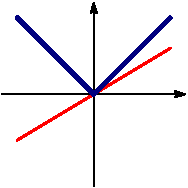
\includegraphics{04absxNoTangent.pdf}}
        \put(  9.33,  17.00){\sffamily\itshape \rotatebox{30.963757}{{\small\sffamily\itshape tangent?}}}
    \put(  8.33,  86.67){\sffamily\itshape \makebox[0pt][c]{$y=|x|$}}
\end{picture}
\\
  The graph of $y=|x|$ has no tangent at the origin}
If we look at the graph of $f(x) = |x|$ then we can see what is wrong:
the graph has a corner at the origin and it is not clear which line,
if any, deserves to be called the tangent line to the graph at the origin.








\subsection{A graph with a cusp. } 
  % !!! Discuss: Change this example to x^{1/3} to make it cleaner?
  Another example of a function without a derivative at $x=0$ is
\[
f(x) = \sqrt{|x|}.
\]%
\marginpar{\footnotesize\sffamily%
  
    \begin{picture} (90.000000,79.000000)(0,0)
    \put(0.0, 0.0){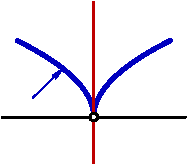
\includegraphics{04sqrtNoTangent.pdf}}
        \put(  1.00,  27.00){\sffamily\itshape $y=\surd{|x|}$}
    \put( 37.00,  48.67){\sffamily\itshape \rotatebox{90}{\small\sffamily\itshape tangent? }}
\end{picture}
\\
  The tangent to the graph of $y=|x|^{1/2}$ at the origin is vertical,
  so its slope is not defined.  The origin is the only
  point on the graph of $y=|x|^{1/2}$ where the tangent is vertical.}%
When you try to compute the derivative you get this limit
\[
f'(0) = \lim_{x\to0} \frac{\sqrt{|x|}}{x} = \text{?}
\]
The limit from the right is
\[
\lim_{x\searrow 0} \frac{\sqrt{|x|}}{x}
= \lim_{x\searrow 0} \frac1{\sqrt x},
\]
which does not exist (it is ``$+\infty$'').  Likewise, the limit from
the left also does not exist (it's ``$-\infty$'').  Nonetheless, a
drawing for the graph of $f$ suggests an obvious tangent line to the graph
at $x=0$, namely the $y$-axis.  That observation does not give us a
derivative, because the $y$-axis is vertical and its slope is not defined.

\begin{figure}
  
    \begin{picture} (360.000000,128.408424)(0,0)
    \put(0.0, 0.0){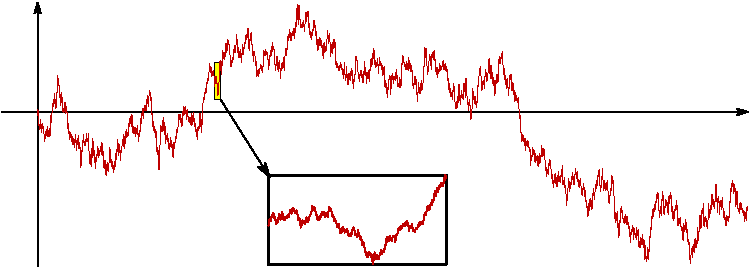
\includegraphics{04brownianMo.pdf}}
        \put(118.14,  64.03){\sffamily\itshape \makebox[0pt][l]{{\rmfamily\itshape\footnotesize(magnify)}}}
    \put(354.74,  78.92){\sffamily\itshape $t$}
    \put( 23.05, 122.29){\sffamily\itshape $x(t)$}
\end{picture}

  \caption{A ``Brownian motion'' provides an example of a function
    $y=f(x)$ that is not differentiable at any $x$.  The graph
    looks like it zig-zags up and down everywhere.  If you magnify any
    small piece of the graph it still has the same jagged appearance. }
\end{figure}

\subsection{A graph with absolutely no tangents, \emph{anywhere}. } 
The previous two examples were about functions that did not have a
derivative at $x=0$.  In both examples the point $x=0$ was the only point
where the function failed to have a derivative.  It is easy to give
examples of functions that are not differentiable at more than one value of
$x$, but here I would like to show you a function $f$ that doesn't have a
derivative \emph{anywhere in its domain.  }

To keep things short I won't write a formula for the function, and merely show
you a graph.  In this graph you see a typical path of a Brownian motion, i.e.\
$t$ is time, and $x(t)$ is the position of a particle which undergoes a Brownian
motion -- come to lecture for further explanation (see also the article on
wikipedia).  To see a similar graph check the Dow~Jones, Nasdaq or S\&P~500 at
the top of the page at \url{http://finance.yahoo.com} in the afternoon on any
weekday.
%\footnote{or at \url{https://www.google.com/finance?client=ob&q=INDEXDJX:DJI}}
% this link is broken
% bummer.


\section{Problems} 
\problemfont 

\begin{multicols}{2}\setlength{\parindent}{0pt}
\noindent%
Compute the derivatives of the following functions,
using either \eqref{eq:derivative-defined} or
\eqref{eq:derivative-defined-a-plus-h}.

\problem $f(x) = x^2-2x $. 
\problem $g(x) = \frac1x $. 
\problem $k(x) = x^3-17x $. 
\problem $u(r) = \frac2{1+r} $. 
\problem $v(\theta) = \sqrt{\theta} $. 
\problem $\varphi(m) = 1/{\sqrt m}$. 
\problem $f(t) = \sqrt[3]{t}$ 
\problem $f(t) = \sqrt{1+2t}$ 
\problem $f(x) = 1/x^2$ 
\problem $f(x) = \sqrt{1+2x} + 1/x^2$ 




\problem Which of the following functions is differentiable at $x=0$? 
\begin{align*}
  f(x) &= x|x|, &g(x) &= x\sqrt{|x|}, \\
  h(x) &= x+|x|, &k(x) &= x^2\sin\frac\pi x,\\
  \ell(x) &= x\sin\frac\pi x.&&
\end{align*}
These formulas do not define $k$ and $\ell$ at $x=0$.  We define $k(0) =
\ell(0) = 0$.

\problem For which value(s) of $a$ and $b$ is the function defined by 
\[
f(x) = \begin{cases}
  ax+b &\text{for $x<0$} \\
  x-x^2 & \text{for $x\geq 0$}
\end{cases}
\]
differentiable at $x=0$?  Sketch the graph of the function $f$ for the
values of $a$ and $b$ you found.

\problem For which value(s) of $a$ and $b$ is the function defined by 
\[
f(x) = \begin{cases}
  ax^2+b &\text{for $x<1$} \\
  x-x^2 & \text{for $x\geq 1$}
\end{cases}
\]
differentiable at $x=1$?  Sketch the graph of the function $f$ for the
values of $a$ and $b$ you found.

\problem For which value(s) of $a$ and $b$ is the function defined by 
\[
f(x) = \begin{cases}
  ax^2 &\text{for $x<2$} \\
  x +b& \text{for $x\geq 2$}
\end{cases}
\]
differentiable at $x=2$?  Sketch the graph of the function $f$ for the
values of $a$ and $b$ you found.

\problem \groupproblem 
\textit{True or false? } If a function $f$ is continuous at some $x=a$
then it must also be differentiable at $x=a$.

\problem \groupproblem 
\textit{True or false? } If a function $f$ is differentiable at some
$x=a$ then it must also be continuous at $x=a$.




\end{multicols}




\noproblemfont
\section{The Differentiation Rules} 
We could go on and compute more derivatives from the definition.  But each time, we
would have to compute a new limit, and hope that there is some trick that allows
us to find that limit.  This is fortunately not necessary.  It turns out that
if we know a few basic derivatives (such as $dx^n/dx=nx^{n-1}$) then we can
find derivatives of arbitrarily complicated functions by breaking them into
smaller pieces.  In this section we look at rules telling us how to
differentiate any function written as either the sum, difference, product or
quotient of two other functions.




\begin{table}[b]
  \centering
  \begin{tabular}[b]
    {l@{\hspace{24pt}}r@{$\,=\,$}l
      @{\hspace{24pt}}r@{$\,=\,$}l}
    \toprule
    \textit{Constant Rule: } & $c'$&$0$ &$\dfrac{dc}{dx}$&$0$ \\[2ex]
%%
    \textit{Sum Rule: } &$(f\pm g)'$&$f'\pm g'$
    &$\dfrac{d}{dx}(f\pm g)$ &$\dfrac{df}{dx}\pm\dfrac{dg}{dx}$ \\[2ex]
%%
    \textit{Product Rule: }
    &$(f\cdot g)'$&$f'\cdot g+f\cdot g'$
    &$\dfrac{d}{dx}(f\cdot g)$ &$\dfrac{df}{dx}\cdot g+f\cdot\dfrac{dg}{dx}$ \\[2ex]
%%
    \textit{Quotient Rule: }
    &$\left(\dfrac{f}{g}\right)'$&$\dfrac{f'\cdot g-f\cdot g'}{g^2}$
    &$\dfrac{d}{dx}\left(\dfrac{f}{g}\right)$
    &$\dfrac{\frac{df}{dx}\cdot g-f\cdot\frac{dg}{dx}}{g^2}$\\[6pt]
    \bottomrule
  \end{tabular}
  \smallskip




  \caption{The differentiation rules:  if you know the derivatives of
    two functions $u(x)$ and $v(x)$, then these rules tell you what
    the derivatives of their sum, product and quotient are.}
  \label{fig:diff-rules}
\end{table}

The situation is analogous to that of the ``limit properties''
$(P_1)$--$(P_6)$ from the previous chapter which allowed us to
compute limits without always having to go back to the formal
definition.

\subsection{Sum, Product, and Quotient Rules} 
In the following, $c$ and
$n$ are constants, $f$ and $g$ are functions of $x$, and ${}'$ denotes
differentiation. The differentiation rules in function notation, and
Leibniz notation, are listed in Table~\ref{fig:diff-rules}.


Note that we already proved the Constant Rule in
\S~\ref{ex:derivative-of-a-constant}.  We will now prove the Sum,
Product and Quotient Rules.

\subsection{Proof of the Sum Rule} 
Suppose that $h(x)=f(x)+g(x)$ for
all $x$ where $f$ and $g$ are differentiable. Then
\begin{align*}
  h'(a)
  & =\lim_{x\to a}\frac{h(x)-h(a)}{x-a}
  &&\textsf{(definition of $h'$)} \\
  & =\lim_{x\to a}\frac{\bigl(f(x)+g(x)\bigr)-\bigl(f(a)+g(a)\bigr)}{x-a}
  &&(\textsf{use }h=f+g)\\
  & =\lim_{x\to a}\left(\frac{f(x)-f(a)}{x-a}+\frac{g(x)-g(a)}{x-a}\right)
  &&\textsf{(algebra)} \\
  & =\left(\lim_{x\to a}\frac{f(x)-f(a)}{x-a}\right)+\left(\lim_{x\to a}\frac{g(x)-g(a)}{x-a}\right)
  &&\textsf{(limit property)} \\[3pt]
  &=f'(a)+g'(a).
  &&\textsf{(definition of $f'$, $g'$)}
\end{align*}






\subsection{Proof of the Product Rule} 
The Product Rule is strange, at
first sight.  In fact, Leibniz first thought that it should look more
like the Sum Rule, and that $(fg)'$ should equal $f'\,g'$.  After
a while he discovered his mistake and figured out that $(fg)' =f'\,g+f\, g'$.  Below is a proof that this rule is correct.  There is
also a picture proof, which we get around to in
\S~\ref{sec:picture-product-rule}.

Let $h(x) = f(x)g(x)$.  To find the derivative we must express the
change of $h$ in terms of the changes of $f$ and $g$:
\begin{align*}
  h(x)-h(a) &= f(x)g(x)-f(a)f(a) \\
  &= f(x)g(x)\underbrace{-f(x)g(a)+f(x)g(a)}_{%
    \makebox[0pt]{\footnotesize\sffamily\centering%
      add and subtract the same term}}
    -f(a)g(a)\\
  &=f(x)\bigl(f(x)-g(a)\bigr) + \bigl(f(x)-g(a)\bigr)v(a)
\end{align*}   
Now divide by $x-a$ and let $x\to a$:
\begin{align*}
  \lim_{x\to a} \frac{h(x)-h(a)}{x-a}
  &= \lim_{x\to a} f(x) \frac{g(x)-g(a)}{x-a} +
  \frac{f(x)-f(a)}{x-a} g(a) \\[1ex]
%  &= \Bigl(\lim_{x\to a} u(x) \Bigr)
%  \Bigl(\lim_{x\to a}\frac{v(x)-v(a)}{x-a} \Bigr)
%  + \Bigl(\lim_{x\to a}\frac{u(x)-u(a)}{x-a} \Bigr)v(a)\\
  &= f(a)g'(a) + f'(a)g(a),
\end{align*}
as claimed.  In this last step we have used that
\[
\lim_{x\to a}\frac{f(x)-f(a)}{x-a} = f'(a)
\quad\text{and}\quad
\lim_{x\to a}\frac{g(x)-g(a)}{x-a} = g'(a)
\]
and also that
\[
\lim_{x\to a} f(x) = u(a)
\]
This last limit follows from the fact that $u$ is continuous,
which in turn follows from the fact that $u$ is differentiable.




  
\subsection{Proof of the Quotient Rule} \label{sec:proof-of-quotient-rule} 
We can break the proof into two parts.  First we do the special case
where $h(x) = 1/g(x)$, and then we use the Product Rule to
differentiate
\[
q(x) = \frac{f(x)}{g(x)} = f(x)\cdot\frac1{g(x)}\;.
\]
So let $h(x) = 1/g(x)$.  We can express the change in $h$ in terms of
the change in $g$:
\[
h(x)-h(a) = \frac1{g(x)} - \frac1{g(a)}
=\frac{g(x)-g(a)}{g(x)g(a)}.
\]
Dividing by $x-a$, we get
\[
\frac{h(x)-h(a)}{x-a} = \frac1{g(x)g(a)} \frac{g(x)- g(a)}{x-a}.
\]
Now we want to take the limit $x\to a$.  We are given that $g$ is
differentiable so it must also be continuous and hence
\[
\lim_{x\to a}g(x) = g(a).
\]
Therefore we find
\[
\lim_{x\to a} \frac{h(x)-h(a)}{x-a} =
\lim_{x\to a}\frac1{g(x)g(a)} \;\lim_{x\to a} \frac{g(x)- g(a)}{x-a}
=\frac{g'(a)}{g(a)^2}.
\]
That completes the first step of the proof.  In the second step,
we use the Product Rule to differentiate $q=f/g$:
\[
q' = \left( \frac fg \right)'
  =\left( f\cdot \frac{1}{g} \right)'
  =f'\cdot\frac{1}{g} + f\cdot\left(  \frac{1}{g}\right)'
=\frac{f'}g - f\frac{g'}{g^2}
=\frac{f'g -fg'}{g^2}.
\]












\subsection{A shorter, but not quite perfect derivation of the Quotient Rule} 
The Quotient Rule can be derived from the Product Rule as follows: for $q=f/g$ then
\begin{equation}\label{eq:quotient-implicity-defined}
  q\cdot g=f
\end{equation}
By the Product Rule, we have
\[
q'\cdot g+q\cdot g'=f',
\]
so that
\[
q' = \frac{f'-q\cdot g'}{g}
= \frac{f'-(f/g)\cdot g'}{g}
=\frac{f'\cdot g-f\cdot g'}{g^2}.
\]
Unlike the proof in \S\ref{sec:proof-of-quotient-rule} above, this argument does
  not prove that $q$ is differentiable if $f$ and $g$ are.
It only says that \emph{if the derivative exists} then it must be what the
Quotient Rule says it is.




The trick we have used here is a special case of a method called ``implicit
differentiation'', which we will discuss much more in
\S~\ref{sec:implicit-differentiation}.




\subsection{Differentiating a constant multiple of a function} 
\label{par:derivative-of-constant-multiple}
Note that the rule
\[
(cf)'=c\,f'
\quad\text{or}\quad
\frac{d\,cu} {dx} = c\, \frac{du} {dx}
\quad\text{or}\quad
\frac{d}{dx}(cf) = c\, \frac{df} {dx}
\]
follows from the Constant Rule and the Product Rule.




\subsection{Picture of the Product Rule} 
  % To write this with f and g instead of u and v, the diagram needs to change
  % in this section.
\label{sec:picture-product-rule}
If $u$ and $v$ are quantities that depend on $x$, and if increasing $x$ by
$\Delta x$ causes $u$ and $v$ to change by $\Delta u$ and $\Delta v$, then the
product of $u$ and $v$ will change by
\begin{equation}
  \label{eq:Delta-uv}
  \Delta(uv)
  =(u+\Delta u)(v+\Delta v) - uv
  = u\Delta v+v\Delta u + \Delta u \Delta v.
\end{equation}
If $u$ and $v$ are differentiable functions of $x$, then the changes $\Delta u$
and $\Delta v$ will be of the same order of magnitude as $\Delta x$, and thus
one expects $\Delta u\Delta v$ to be much smaller.  One therefore ignores the
last term in \eqref{eq:Delta-uv}, and thus arrives at
\[
\Delta(uv) =  u\Delta v+v\Delta u.
\]
Leibniz would now divide by $\Delta x$ and replace $\Delta$'s by $d$'s
to get the Product Rule:
\[
\frac{\Delta(uv)}{\Delta x}
=  u\frac{\Delta v}{\Delta x}+v\frac{\Delta u}{\Delta x}.
\]
\begin{figure}[h]\centering
  
    \begin{picture} (200.000000,158.750000)(0,0)
    \put(0.0, 0.0){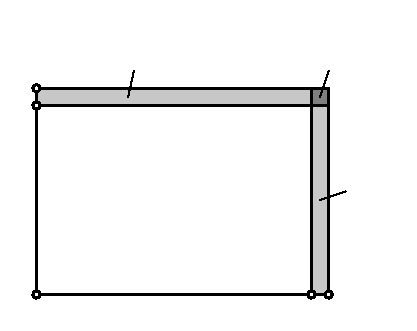
\includegraphics{04prodRulePicture.pdf}}
        \put( 83.50,   5.50){\sffamily\itshape \makebox[0pt][c]{$u$}}
    \put(153.62,   5.50){\sffamily\itshape \makebox[0pt][c]{$\Delta u$}}
    \put( 14.50,  62.87){\sffamily\itshape \makebox[0pt][r]{$v$}}
    \put( 14.50, 112.37){\sffamily\itshape \makebox[0pt][r]{$\Delta v$}}
    \put( 83.50,  62.87){\sffamily\itshape \makebox[0pt][c]{$uv$}}
    \put(168.00,  67.00){\sffamily\itshape \makebox[0pt][l]{$v\Delta u$}}
    \put( 64.25, 126.75){\sffamily\itshape \makebox[0pt][c]{$u\Delta v$}}
    \put(157.75, 126.75){\sffamily\itshape \makebox[0pt][c]{$\Delta u\Delta v$}}
\end{picture}

  \caption{The Product Rule. \textit{How much does the area of a rectangle
  change if its sides $u$ and $v$ are increased by $\Delta u$ and
  $\Delta v$? } Most of the increase is accounted for by the two thin
  rectangles whose areas are $u\Delta v$ and $v\Delta u$.  So the increase
  in area is approximately $u\Delta v + v\Delta u$, which explains why the
  product rule says $(uv)' = uv'+ vu'$. }
\end{figure}




\section{Differentiating powers of functions} 
% !!! Evan did not bother fixing typos here since he wants to delete this entire section, for being just special cases of the chain rule
\subsection{Product rule with more than one factor} 
If a function is given as the product of $n$ functions, i.e.
\[
f(x) = u_1(x) \times u_2(x) \times \cdots \times  u_n(x),
\]
then you can differentiate it by applying the product rule $n-1$ times
(there are $n$ factors, so there are $n-1$ multiplications.)




In the first step you write $f(x)$ as the product of two functions
\[
f(x) = u_1(x) \times \bigl(u_2(x)u_3(x)\cdots u_n(x)\bigr),
\]
would get
\[
f' = u_1' \bigl(u_2\cdots u_n\bigr) + u_1\bigl(u_2\cdots u_n\bigr)'.
\]
In the second step you apply the product rule to $(u_2u_3\cdots
u_n)'$.  This yields
\begin{align*}
  f'
  &= u_1' u_2\cdots u_n + u_1\bigl[u_2'u_3\cdots u_n+u_2(u_3\cdots
  u_n)'\bigr]\\
  &= u_1'u_2\cdots u_n + u_1u_2'u_3\cdots u_n + u_1u_2\bigl(u_3\cdots
  u_n\bigr)'.
\end{align*}
Continuing this way one finds after $n-1$ applications of the product rule
that
\begin{equation}
  \label{eq:product-rule-n-factors}
  \bigl(u_1\cdots u_n\bigr)'
  = u_1'u_2\cdots u_n + u_1u_2'u_3\cdots u_n +\, \cdots\, + u_1u_2u_3\cdots
  u_n'.
\end{equation}








\subsection{The Power rule} 
  % !!! Discuss: delete this section too
If all $n$ factors in the previous paragraph are the same, i.e.\ $u_1(x) =
u_2(x) = \cdots = u_n(x) = u(x)$, then the function $f$ is the
$n^{\text{th}}$ power of some other function,
\[
f(x) = \bigl(u(x)\bigr)^n.
\]
If we use the product rule to find the derivative of $f(x)$, we find that
all terms in the right hand side of \eqref{eq:product-rule-n-factors} are
the same.  Since there are $n$ of them, we get
\[
f'(x) = n\, u(x)^{n-1}\, u'(x),
\]
or, in Leibniz' notation,
\begin{equation}
  \label{eq:Power-rule}
  \frac{du^n}{dx} = nu^{n-1}\frac{du}{dx}.
\end{equation}












\subsection{The Power Rule for Negative Integer Exponents} 
    % !!! Discuss: move this to where the power rule is initially discussed and
    % simply say that the negative exponent case also holds, but without
    % providing a proof there.
We have just proved the power rule \eqref{eq:Power-rule} assuming $n$ is a
positive integer.  The rule actually holds for all real exponents $n$, but
the proof is harder.  




Here we prove the Power Rule for negative exponents using the Quotient
Rule.  Suppose $n=-m$ where $m$ is a positive integer.   Then the Quotient
Rule tells us that
\[
(u^n)'
=\bigl(u^{-m}\bigr)'
=\left(\frac{1}{u^m}\right)'
\stackrel{\text{Q.R.}}{=}
-\frac{(u^m)'}{(u^m)^2}.
\]
Since $m$ is a positive integer, we can use \eqref{eq:Power-rule}, so
$(u^m)' = mu^{m-1}$, and hence
\[
(u^n)'
= -\frac{mu^{m-1}\cdot u'}{u^{2m}}
=-mu^{-m-1}\cdot u'
= n u^{n-1}u'.
\]








\subsection{The Power Rule for Rational Exponents} 
      % !!! Discuss: move this to where the power rule is initially discussed and simply say that the negative exponent case also holds, but without providing a proof there.
      % !!! Issue: this application of implicit differentiation is totally bogus
      % (without having covered implicit differentiation yet).
So far we have proved that the power law holds if the exponent $n$ is an
integer.




We now show that the power law holds even if the exponent $n$ is any
fraction, $n=p/q$.  The following derivation contains the trick called
\emph{implicit differentiation} which we will study in more detail in
Section~\ref{sec:implicit-differentiation}.




So let $n=p/q$ where $p$ and $q$ are integers and consider the function
\[
w(x)=u(x)^{p/q}.
\]
Assuming that both $u$ and $w$ are differentiable functions, we will show that
\begin{equation}\label{eq:power-rule-rational-exponents}
  w'(x) = \frac pq u(x)^{\frac pq-1}u'(x)
\end{equation}








Raising both sides to the $q$th power gives
\[
w(x)^q=u(x)^p.
\]
Here the exponents $p$ and $q$ are integers, so we may apply the Power Rule
to both sides.  We get
\[
qw^{q-1}\cdot w'=pu^{p-1}\cdot u'.
\]
Dividing both sides by $qw^{q-1}$ and substituting $u^{p/q}$ for $w$ gives
\[
w'= \frac{pu^{p-1}\cdot u'}{qw^{q-1}}=
\frac{pu^{p-1}\cdot u'}{qu^{p(q-1)/q}}=
\frac{pu^{p-1}\cdot u'}{qu^{p-(p/q)}}=
\frac{p}{q}\cdot u^{(p/q)-1}\cdot u'
\]
which is the Power Rule for $n=p/q$.








This proof is flawed because we did not show that $w(x) = u(x)^{p/q}$ is
differentiable:  we only showed what the derivative should be,
\textit{if it exists. }
















\subsection{Derivative of $x^n$ for integer $n$} 
  % This is beyond pointless to include here!!!
If you choose the function $u(x)$ in the Power Rule to be $u(x) = x$, then
$u'(x) = 1$, and hence the derivative of $f(x) = u(x)^n = x^n$ is
\[
f'(x)
= nu(x)^{n-1} u'(x)
= nx^{n-1}\cdot 1
= nx^{n-1}.
\]
We already knew this of course.












\subsection{Example -- differentiate a polynomial} 
Using the Differentiation Rules we can easily differentiate any polynomial and
hence any rational function.  For example, using the Sum Rule, the Power Rule,
and the rule $(cu)'=cu'$, we see that the derivative of the polynomial
\[
f(x)= 2x^4-x^3+7
\]
is
\[
f'(x)=8x^3-3x^2.
\]




\subsection{Example -- differentiate a rational function} 
By the Quotient Rule the derivative of the function
\[
g(x)=\frac{2x^4-x^3+7}{1+x^2}
\]
is
\begin{align*}
  g'(x)&=\frac{(8x^3-3x^2)(1+x^2)-(2x^4-x^3+7)2x}{(1+x^2)^2}\\
  &=\frac{6x^5-x^4+8x^3-3x^2-14x}{(1+x^2)^2}.
\end{align*}
By comparing this example with the previous one, it seems to be the case that
polynomials simplify when we differentiate them, while rational
functions become more complicated.




\subsection{Derivative of the square root} 
The derivative of $f(x)=\sqrt{x}=x^{1/2}$ is
\[
f'(x)
= \frac12 x^{1/2 -1}
= \frac12 x^{-1/2}
= \frac1{2x^{1/2}}=\frac1{2\sqrt x}
\]
where we used the Power Rule with $n=1/2$ and $u(x)=x$.








\section{Problems} 
\problemfont 
\begin{multicols}{2}\setlength{\parindent}{0pt}
\problem Let $f(x)=(x^2+1)(x^3+3)$. Find $f'(x)$ in two ways:\\ 
\textbf{(a)}~by multiplying and then differentiating, \\
\textbf{(b)}~by using the Product Rule.\\
Are your answers the same?








\problem  Let $f(x)=(1+x^2)^4$. Find $f'(x)$ in two ways, first by 
expanding to get an expression for $f(x)$ as a polynomial in $x$ and
then differentiating, and then by using the Power Rule.  Are the
answers the same?








\problem Prove the statement in \S\ref{par:derivative-of-constant-multiple}, that $(cu)' = c(u')$ follows from the Product Rule. 








\noindent \textit{Compute the derivatives of the following functions}
(Try to simplify your answers.)\\




\problem $\DS f(x) = x+1+(x+1)^2$ 




\problem $\DS f(x) = \frac{x-2}{x^4+1}$ 




\problem $\DS f(x) = \left(\frac{1}{1+x}\right)^{-1}$ 




\problem $\DS f(x) = \sqrt{1-x^2}$ 




\problem $\DS f(x) = \frac{ax+b}{cx+d}$ 




\problem $\DS f(x) = \frac1{(1+x^2)^2}$ 




\problem $\DS f(x) = \frac{x}{1+\sqrt x}$ 




\problem $\DS f(x) = \sqrt{\frac{1-x}{1+x}}$ 




\problem $\DS f(x) = \sqrt[3]{x+\sqrt x}$ 




\problem $\DS \varphi(t) = \frac{t}{1+\sqrt t} $ 




\problem $\DS g(s) = \sqrt{\frac{1-s}{1+s}} $ 




\problem $\DS h(\rho) = \sqrt[3]{\rho+\sqrt \rho}$ 












\problem \groupproblem\textit{Using derivatives to approximate numbers. } 




\subprob Find the derivative of $f(x) = x^{4/3}$.




\subprob Use \textbf{(a)} to estimate the number
\[
\frac{127^{4/3}-125^{4/3}}{2}
\]
approximately without a calculator. Your answer should have the form
$p/q$ where $p$ and $q$ are integers.  [\textsl{Hint: Note that
$5^3=125$ and take
a good look at equation \eqref{eq:derivative-defined}.}]




\subprob Approximate in the same way the numbers $\sqrt{99}$ and
$\sqrt{101}$. (Hint: $10\times 10=100$.)








\problem\label{ex:05log-derivs} 
  % This problem shouldn't be here, it should be later with logs and exponentials!
\textit{(Making the Product and Quotient rules look nicer)}




Instead of looking at the derivative of a function you
can look at the ratio of its derivative to the function itself, i.e.\
you can compute $f'/f$.  This quantity is called the
\emph{logarithmic derivative of the function $f$} for reasons that
will become clear later this semester.
% add forward reference to logs section


\subprob Compute the logarithmic derivative of these functions (i.e., find
$f'(x)/f(x)$):
\begin{gather*}
  f(x) = x ,\quad g(x) =3x ,\\
  h(x) =x^2 \quad k(x) =-x^2 ,\\
  \ell(x) =2007x^2,\quad m(x) =x^{2007}
\end{gather*}




\subprob Show that for any pair of functions $u$ and $v$ one has
\begin{align*}
  \frac{(uv)'}{uv} &= \frac{u'}{u} + \frac{v'}{v}\\
  \frac{(u/v)'}{u/v} &= \frac{u'}{u} - \frac{v'}{v}\\
  \frac{\bigl(u^n\bigr)'}{u^n} &= n\; \frac{u'}{u}
\end{align*}
















\problem   
\subprob Find $f'(x)$ and $g'(x)$ if
\[
f(x)=\frac{1+x^2}{2x^4+7}, \qquad g(x)=\frac{2x^4+7}{1+x^2}.
\]
Note that $f(x)=1/g(x)$.\\
\subprob Is it true that $f'(x)=1/g'(x)$?\\
\subprob Is it true that $f(x) = g^{-1}(x)$?\\
\subprob Is it true that $f(x)= g(x)^{-1}$?\\








\problem \subprob Let 
\begin{gather*}
  x(t)=(1-t^2)/(1+t^2),\\
  y(t)=2t/(1+t^2),\\
  u(t)=y(t)/x(t).
\end{gather*}
Find $dx/dt$, $dy/dt$.




\subprob Now that you've done \textbf{(a)} there are two
different ways of finding $du/dt$.  Do
both of them, and compare the results you get.




\end{multicols}
\normalsize\rmfamily








\noproblemfont
\section{Higher Derivatives} 




\subsection{The derivative of a function is a function} 
If the derivative $f'(a)$ of some function $f$ exists for all $a$ in the domain
of $f$, then we have a new function: namely, for each number in the domain of
$f$ we compute the derivative of $f$ at that number.  This function is called
the \emph{derivative function} of $f$, and it is denoted by $f'$.  Now that we
have agreed that the derivative of a function is a function, we can repeat the
process and try to differentiate the derivative.  The result, if it exists, is
called the \emph{second derivative of $f$}.  It is denoted $f''$.  The
derivative of the second derivative is called the third derivative, written
$f'''$, and so on.




The $n$th derivative of $f$ is denoted $f^{(n)}$.  Thus
\[
f^{(0)}=f,\qquad f^{(1)}=f',\qquad f^{(2)}=f'',\qquad
f^{(3)}=f''',\ldots.
\]
Leibniz' notation for the $n$th derivative of $y=f(x)$ is
\[
\frac{d^ny}{dx^n}= f^{(n)}(x).
\]








\subsection{Two examples} 
If $f(x) = x^2-2x+3$ and $g(x) = x/(1-x)$ then
\begin{align*}
  f(x) &= x^2 - 2x + 3  & g(x)&= \frac{x} {1-x} \\
  f'(x) &= 2x -2 & g'(x) &= \frac{1} {(1-x)^2} \\
  f''(x) &= 2 & g''(x) &= \frac{2} {(1-x)^3} \\
  f^{(3)}(x) &= 0 & g^{(3)}(x) &= \frac{2\cdot 3} {(1-x)^4}\\
  f^{(4)}(x) &= 0 & g^{(4)}(x) &= \frac{2\cdot3\cdot4} {(1-x)^5}\\
  &\vdots &&\vdots
\end{align*}
All further derivatives of $f$ are zero, but no matter how often we
differentiate $g(x)$ we will never get zero.  Instead of multiplying the
numbers in the numerator of the derivatives of $g$ we left them as
``$2\cdot3\cdot4$.''  A good reason for doing this is that we can see
a pattern in the derivatives, which would allow us to guess what (say) the
$10$th derivative is, without actually computing ten derivatives:
\[
g^{(10)}(x) =
\frac{2\cdot3\cdot4\cdot5\cdot6\cdot7\cdot8\cdot9\cdot10} {(1-x)^{11}}.
\]








\subsection{Operator notation} 
  % added discussion of operator notation earlier that repeats some of this
\label{sec:04operator-notation}
A common variation on Leibniz notation for derivatives is the so-called
\emph{operator notation}, as in
\[
\frac{d(x^3-x)}{dx} = \frac{d}{dx} (x^3-x)= 3x^2-1.
\]
For higher derivatives one can write
\[
\frac{d^2y}{dx^2}
= \frac{d} {dx} \frac{d} {dx}y
= \left(\frac{d}{dx}\right)^2 y
\]
Be careful to distinguish the second derivative from the square of the first
derivative. Usually
\[
\frac{d^2y}{dx^2}\ne\left(\frac{dy}{dx}\right)^2\text{\large\bfseries!!!!}
\]




\section{Problems} 
\problemfont 




\begin{multicols}{2}\setlength{\parindent}{0pt}
\problem  The equation 
\begin{equation}
  \frac{2x}{x^2-1}= \frac{1}{x+1}+\frac{1}{x-1}  \tag{\dag}
\end{equation}
holds for all values of $x$ (except $x=\pm1$), so you should get
the same answer if you differentiate both sides.  Check this.




Compute the third derivative of $f(x) = 2x/(x^2-1)$ by using either the
left or right hand side (your choice) of (\dag).




\problem Compute the first, second and third derivatives of the following 
functions:




\subprob $f(x) = (x+1)^4$




\subprob $g(x) = \bigl(x^2+1\bigr)^4$




\subprob $h(x) = \sqrt{x-2} $




\subprob $k(x) = \sqrt[3]{x-\frac1x}$
















\problem Find the derivatives of $10^\text{th}$ order of the following 
functions. (The problems have been chosen so that after doing the
first few derivatives in each case, you should start seeing a pattern
that will let you guess the $10^{\text{th}}$ derivative without
actually computing $10$ derivatives.)




\subprob $  f(x) = x^{12}+x^8 $.




\subprob $  g(x) = 1/x $.




\subprob $  h(x) = 12/(1-x)$.




\subprob $  k(x) = x^2/(1-x)$.




\subprob $  \ell(x) = 1/(1-2x)$




\subprob $  m(x) = x/(1+x)$








\problem 
Find $f'(x)$, $f''(x)$ and $f^{(3)}(x)$ if
\[
f(x)=1+x+\frac{x^2}{2}+\frac{x^3}{6}+\frac{x^4}{24}
+\frac{x^5}{120}+\frac{x^6}{720}.
\]








\problem \groupproblem  Suppose we have these two functions 
\[
f(x)=\frac{1} {x+2},\quad
g(x)=\frac{x} {x+2}.
\]




\subprob  Find the 12$^{\text{th}}$ derivative of $f(x)$.




\subprob  Find the $n^{\text{th}}$ order derivative of
$f(x)$  (i.e.\ find a formula for $f^{(n)}(x)$
which is valid for all $n=0, 1, 2, 3\ldots$).




\subprob  Find the $n^{\text{th}}$ order derivative of
$g(x)$.




\subprob Find $h^{(n)}(x)$ where $h(x) = \dfrac{x^2} {x+2}$.
















\problem \groupproblem \textit{(Mostly about notation)} 




\subprob  Find $dy/dx$ and $d^2y/dx^2$ if $y= x/( x+2)$.  




\subprob  Find $du/dt$ and $d^2u/dt^2$ if $u= t/(t+2)$.




\subprob  Find $\DS \frac{d}{dx}\left(\frac x{x+2}\right)$ and
$\DS\frac{d^2}{dx^2}\left(\frac x{x+2}\right)$.  




\subprob  Compute
\[
A= \frac{d\dfrac{x} {x+2}} {dx} \text{ at $x=1$,}
\]
and
\[
B= \frac{d\dfrac{1} {1+2}} {dx}\;.
\]
\answer 
The derivative of $x/(x+2)$ is $2/(x+2)^2$, so the derivative at $x=1$ is
$A = \frac29$.




On the other hand
$1/(1+2) = \frac13$ is constant, so its derivative is $B=0$.
\endanswer




\subprob Simplicio just thought of this argument:
\textit{if you set $x=1$ in $x/(x+2)$ you get
$1/(1+2)$; therefore these two quantities have the same derivative when
$x=1$, and hence in the previous problem you should have found $A=B$. }




Is he right?  What do you conclude from his reasoning?
\answer 
Simplicio is mistaken.  The mistake is that he assumes that setting $x$
equal to some constant and then differentiating gives the same result as first
differentiating w.r.t.~$x$ and then setting $x$ equal to some constant.  This
example shows that is not true.
\endanswer








\problem  \label{ex:d2ydx2dydx2} Find $d^2y/dx^2$ and 
$(dy/dx)^2$ if $y=x^3$.




















\end{multicols}
\noproblemfont
\section{Differentiating trigonometric functions} 
\label{sec:trigDerivatives}
The trigonometric functions sine, cosine and tangent are differentiable, and
their derivatives are given by the following formulas
\begin{equation}
  \frac{d\sin x}{dx} = \cos x,\quad
  \frac{d\cos x}{dx} = -\sin x,\quad
  \frac{d\tan x}{dx} = \frac1{\cos^2 x}.
\end{equation}
Note the minus sign in the derivative of the cosine!




\subsection{The derivative of $\sin x$} 
\label{sec:deriv-deriv-sin}
By definition one has
\begin{equation}\label{eq:derivation-of-deriv-of-sine}
  \sin'(x)=\lim_{h\to 0}\frac{\sin(x+ h)-\sin(x)}{h} .
\end{equation}
To simplify the numerator we use the trigonometric addition formula
\[
\sin(\alpha+\beta) = \sin\alpha\cos\beta+\cos\alpha\sin\beta.
\]
with $\alpha=x$ and $\beta=h$, which results in
\begin{align*}
  \frac{\sin(x+ h)-\sin(x)}{h} &=
  \frac{\sin(x)\cos(h)+\cos(x)\sin(h)-\sin(x)}{h}\\
  &= \cos(x)\frac{\sin(h)}{h}+\sin(x)\frac{\cos(h)-1}{h}
\end{align*}
Hence by the formulas
\[
\lim_{h\to 0}\frac{\sin(h)}{h} = 1 \qquad\mbox{ and }\qquad
\lim_{h\to 0}\frac{\cos (h)-1}{h} = 0
\]
from Chapter~III, \S~\ref{sec:trigLimit} we have
\begin{align*}
  \sin'(x)
  &= \lim_{h\to 0} \cos(x)\frac{\sin(h)}{h}+\sin(x)\frac{\cos(h)-1}{h}\\
  &= \cos(x) \cdot 1 + \sin(x) \cdot 0\\
  &= \cos(x).
\end{align*}




A similar computation leads to the stated derivative of $\cos x$.




To find the derivative of $\tan x$ we apply the Quotient Rule to
\[
\tan x=\frac{\sin x}{\cos x} = \frac{f(x)}{g(x)}.
\]
We get
\[
\tan'(x)=\frac{\cos(x)\sin'(x) - \sin(x) \cos'(x)}{\cos^2(x)}
=\frac{\cos^2(x)+\sin^2(x)}{\cos^2(x)} =\frac{1}{\cos^2(x)}
\]
as claimed.








\section{Problems} 
\problemfont 
\begin{multicols}{2}\setlength{\parindent}{0pt}
\noindent Find the derivatives of the following functions (try to simplify
your answers)




\problem $\DS f(x) = \sin(x) + \cos(x) $ 




\problem $\DS f(x) = 2\sin(x) - 3\cos(x) $ 




\problem $\DS f(x) = 3\sin(x) + 2\cos(x) $ 




\problem $\DS f(x) = x\sin(x) + \cos(x) $ 




\problem $\DS f(x) = x\cos(x) -\sin x $ 




\problem $\DS f(x) = \frac{\sin x}{x} $ 




\problem $\DS f(x) = \cos^2(x) $ 




\problem $\DS f(x) = \sqrt{1-\sin^2 x} $ 




\problem $\DS f(x) = \sqrt{\frac{1-\sin x}{1+\sin x}} $ 




\problem $\DS \cot(x) = \frac{\cos x}{\sin x}.$ 




\problem Can you find $a$ and $b$ so that the function 
\[
f(x) = \begin{cases}
  \cos x & \text{for $x\leq \frac\pi4$} \\
  a+bx   & \text{for $x > \frac\pi4$}
\end{cases}
\]
is differentiable at $x=\pi/4$?








\problem Can you find $a$ and $b$ so that the function 
\[
f(x) = \begin{cases}
  \tan x & \text{for $x< \frac\pi4$} \\
  a+bx   & \text{for $x\geq\frac\pi4$}
\end{cases}
\]
is differentiable at $x=\pi/4$?




\problem  Show that the functions 
\[
f(x) = \sin^2 x \text{ and } g(x) = -\cos^2x
\]
have the same derivative by computing $f'(x)$ and $g'(x)$.




With hindsight this was to be expected -- why?




\problem Simplicio claims that our formula for the derivative of $\tan x$ must 
be wrong because he has a book that says
\[
\frac{d\tan x} {dx} = 1+\tan^2 x.
\]
Show that both formulas are right.




\problem Find the first, second and third derivatives of the functions 
\[
f(x) = \tan^2 x \text{ and }
g(x) = \frac{1}{\cos^2 x}.
\]
Hint: remember your trig to reduce work!
\answer 
$f'(x) = 2\tan x/\cos^2 x$




$f''(x) = 2/\cos^4 x + 4\tan x \sin x/\cos^3 x$




$f'''(x) = -8\sin x/\cos^8 x + 4\sin x/\cos^5 x
           + 4\tan x/\cos^2x - 12\tan x \sin^2x/\cos^6x$.




Since $\tan^2 x= \frac{1}{\cos^2 x}-1$ one has $g'(x) = f'(x)$ and
$g''(x) = f''(x)$.
\endanswer




\problem \textit{A geometric derivation of the derivatives of sine and cosine.} 




\centerline{\input ../figures/221/03sine-derivative.pdf_tex}




In the lower picture you see a unit circle, a point $P$ with angle $ \theta $, whose
coordinates are $(\cos \theta, \sin \theta)$.  The figure also shows the point $Q$
you get if you increase the angle $\theta$ by a small amount
$\Delta\theta$. Drawing horizontal and vertical lines through these two points
then produces the shaded triangular area.  The picture above the circle is a
magnification of the shaded triangle.  The hypotenuse of the triangle is not
straight since it is part of the unit circle, but the smaller you make
$\Delta\theta$ the closer it will be to a straight line segment.  The lengths of
the sides of the triangle are $\Delta\theta$, the change in $\sin\theta$ and the
change of $\cos \theta$.  Since it is a right triangle you can express
\[
\frac{\Delta\sin \theta} {\Delta\theta} \text{ and }
\frac{\Delta\cos\theta} {\Delta\theta}
\]
as the sine and/or cosine of some angle.  Find the relevant angle, and show how this
leads to our formulas for the derivatives of $\sin\theta$ and $\cos\theta$.




Make sure you explain where the ``$-$'' in the derivative of $\cos\theta$ comes from.




\problem \groupproblem \textit{(Yet another derivation of the formula for 
$d\sin x / dx$)}




In \S~\ref{sec:deriv-deriv-sin} above we used the addition formula for
$\sin(\alpha+\beta)$ to compute the limit
(\ref{eq:derivation-of-deriv-of-sine}).  Instead of using the addition
formula, use this formula from trigonometry
\[
\sin\alpha - \sin\beta
=
2\sin \bigl(\frac{\alpha-\beta} {2}\bigr) \cos\bigl(\frac{\alpha+\beta} {2}\bigr)
\]
to compute the limit (\ref{eq:derivation-of-deriv-of-sine}).




\end{multicols}












\noproblemfont
\section{The Chain Rule} 
\subsection{Composition of functions} 
Given two functions $f$ and $g$, we can define a new function called
the \emph{composition of $f$ and $g$}.  The notation for the
composition is $f\circ g$, and it is defined by the formula
\[
f\circ g(x)  = f\bigl(g(x)\bigr).
\]
The domain of the composite function is the set of all numbers $x$ for which
this formula gives we something well-defined.




If you think of functions as expressing dependence of one quantity on another,
then the composition of functions arises as follows:  If a quantity $z$ is a
function of another quantity $y$, and if $y$ itself depends on $x$, then $z$
depends on $x$ via $y$.  See Figure~\ref{fig:04growing-balloon} for a concrete
example of such a chain of dependencies, and thus of composing two functions.












\begin{figure}[t]




  \noindent\rule{\textwidth}{1pt}




  \begin{minipage}[b]{\textwidth}\sffamily\color{darkbluegreen}
    \setlength{\parindent}{1pc}
    \rule{0pt}{12pt}\centerline{\sffamily\bfseries%
      A depends on B depends on C depends on\ldots}
    \begin{multicols}{2}
      \noindent\small%
      Someone is pumping water into a balloon.  Assuming that the balloon is a
      sphere, we can say how large it is by specifying its radius $R$.  For an
      expanding balloon this radius will change with time $t$.




      The volume of the balloon is a function of its radius, since the
      volume of a sphere of radius $R$ is given by
      \[ V=\frac43\pi
      R^3.\]
      We now have two functions: the first ($f$) tells
      us the radius $R$ of the balloon at time $t$,
      \[
        R=f(t),
      \]
      and the second function ($g$) tells us the volume of the balloon given
      its radius
      \[
        V=g(R).
      \]
      The volume of the balloon at time $t$ is then given by
      \[
        V=g\bigl(f(t)\bigr) = g\circ f(t),
      \]
      and it is the function that tells us the volume of the balloon at time
      $t$, and is the composition of first $f$ and then $g$.




      Schematically we can summarize this chain of cause-and-effect relations as
      follows: we could either say that $V$ depends on $R$, and $R$ depends on
      $t$,
      \[
      \text{\framebox{\parbox{3em}{\centering\footnotesize%
              time $t$}}}
      \stackrel{\DS f}{\longrightarrow}
      \text{\framebox{\parbox{4em}{\centering\footnotesize%
      radius $R$\\
      depends on time $t$} }}
      \stackrel{\DS g}{\longrightarrow}
      \text{\framebox{\parbox{4em}{\centering\footnotesize%
      volume $V$\\ depends on radius $R$} }}
      \]
      or we could say that $V$ depends directly on $t$:
      \[
      \text{\framebox{\parbox{3em}{\centering\footnotesize%
              time $t$}}} \; \;
      \stackrel{\DS g\circ f}{\longrightarrow }\; \;
      \text{\framebox{\parbox{6em}{\centering\footnotesize%
      volume~$V$\\ depends on\\ time $t$}}}
      \]
    \end{multicols}




    \rule{0pt}{6pt}




  \end{minipage}




  \noindent\rule{\textwidth}{1pt}




  \caption{A ``real world example'' of a composition of functions.}
  \label{fig:04growing-balloon}
\end{figure}




\subsection{Example} 
\label{sec:04composition-example}
Suppose we have three quantities, $x$, $y$, and $z$ which are related by
\[
z=y^2+y, \text{ and } y = 2x+1.
\]
Here we have a chain of dependencies, with $z$ depending on $y$ and $y$
depending on $x$.  By combining (composing) these dependencies you see that $z$
depends on $x$ via
\[
z = y^2+y = (2x+1)^2 + 2x+1.
\]




We can express the same ideas in function notation.  The first dependency
$z=y^2+y$ defines a function, which we'll call $f$.  It is given by
\[
f(y) = y^2+y.
\]
The second dependency, $y=2x+1$, also defines a function
\[
g(x) = 2x+1.
\]
The way the quantity $z$ depends on $x$ also defines a function, namely,
the composition of $f$ and $g$.  The composition is
\[
f\circ g(x) =f\bigl(2x+1\bigr) = (2x+1)^2+(2x+1)
\]
In other notation,
\[
\left.
\begin{array}{cc}
z=f(y) \\ y = g(x)
\end{array}
\right\}
\implies z = f\bigl(g(x)\bigr) = f\circ g(x).  
\]
One says that \emph{the composition of $f$ and $g$ is the result of
substituting $g$ in $f$}.




\medskip




How can we find the derivative of the composition of two functions?  This is
what the Chain Rule tells us:


\subsection{Theorem (Chain Rule)} 
\label{thm:chainRule}\itshape
If $f$ and $g$ are differentiable, so is the composition $f\circ g$.




The derivative of $f\circ g$ is given by
\[
(f\circ g)'(x) = f'(g(x))\;g'(x).
\]\upshape








The Chain Rule looks a lot simpler, perhaps even ``obvious'', if we write it in
Leibniz notation.  Let's translate from function notation to ``$d\text{this}
/d\text{that}$'':




Suppose that $y=g(x)$ and $z=f(y)$, then $z=f\circ g(x)$, and
the derivative of $z$ with respect to $x$ is the derivative of the function
$f\circ g$.  The derivative of $z$ with respect to $y$ is the derivative of the
function $f$, and the derivative of $y$ with respect to $x$ is the derivative of
the function $g$.  In short,
\[
\frac{dz}{dx} =(f\circ g)'(x),\quad
\frac{dz}{dy} = f'(y) \quad\text{and }
\frac{dy}{dx} = g'(x)
\]
so now the Chain Rule says
\begin{equation}\label{eq:chainrule-ala-Leibniz}
  \frac{dz}{dx} = \frac{dz}{dy} \; \frac{dy}{dx}.
\end{equation}
\subsection{First proof of the Chain Rule (using Leibniz notation)} 




We first consider difference quotients instead of derivatives, i.e.\ using the
same notation as above, we consider the effect of an increase of $x$ by an
amount $\Delta x$ on the quantity $z$.




If $x$ increases by $\Delta x$, then $y=g(x)$ will increase by
\[
\Delta y = g(x+\Delta x) - g(x),
\]
and $z=f(y)$ will increase by
\[
\Delta z = f(y+\Delta y) -f(y).
\]
The ratio of the increase in $z=f(g(x))$ to the increase in $x$ is
\[
\frac{\Delta z}{\Delta x} = \frac{\Delta z}{\Delta y} \;\cdot\; \frac{\Delta
  y}{\Delta x}.
\]
In contrast to $dx$, $dy$ and $dz$ in equation \eqref{eq:chainrule-ala-Leibniz},
the $\Delta x$, etc.\ here are finite quantities, so this equation is just
algebra: you can cancel the two $\Delta y$s.  If you let the increase $\Delta x$
go to zero, then the increase $\Delta y$ will also go to zero, and the
difference quotients converge to the derivatives,
\[
\frac{\Delta z}{\Delta x} \longrightarrow \frac{dz}{dx},\quad \frac{\Delta
  z}{\Delta y} \longrightarrow \frac{dz}{dy},\quad \frac{\Delta y}{\Delta x}
\longrightarrow \frac{dy}{dx}
\]
which immediately leads to Leibniz's form of the Chain Rule.
 


\subsection{Second proof of the Chain Rule} 
We verify the formula in Theorem \ref{thm:chainRule} at some arbitrary value
$x=a$.  Specifically, we will show that
\[
(f\circ g)'(a) = f'(g(a))\;g'(a).
\]
By definition the left hand side is
\[
(f\circ g)'(a) = \lim_{x\to a}\frac{(f\circ g)(x)-(f\circ g)(a)}{x-a} =
\lim_{x\to a}\frac{f(g(x))-f(g(a))}{x-a}.
\]
The two derivatives on the right hand side are given by
\[
g'(a) = \lim_{x\to a} \frac {g(x)- g(a)}{x-a}
\]
and
\[
f'(g(a)) = \lim_{y\to g(a)} \frac{f(y) - f(g(a))}{y-g(a)}.
\]
Since $g$ is a differentiable function it must also be a continuous function,
and hence $\lim_{x\to a} g(x) = g(a)$.  So we can substitute $y=g(x)$ in the
limit defining $f'(g(a))$
\begin{equation}
  f'(g(a)) = \lim_{y\to g(a)} \frac{f(y) - f(g(a))}{y-g(a)}
  =\lim_{x\to a} \frac{f(g(x))-f(g(a))}{g(x)-g(a)}.  
\end{equation}
(Keep in mind that as $x\to a$ one has $y\to g(a)$.)  By putting all this
together, we get
\begin{align*}
  (f\circ g)'(a)
  &= \lim_{x\to a}\frac{f(g(x))-f(g(a))}{x-a}\\
  &= \lim_{x\to a}
  \frac{f(g(x))-f(g(a))}{g(x)-g(a)}\cdot\frac{g(x)-g(a)}{x-a}\\
  &= \lim_{x\to a} \frac{f(g(x))-f(g(a))}{g(x)-g(a)}
  \cdot\lim_{x\to a}\frac{g(x)-g(a)}{x-a}\\
  &=f'(g(a)) \;\cdot\;g'(a)
\end{align*}
which is what we were supposed to prove -- the proof \textit{seems} complete.




There is one flaw in this proof, namely, we have divided by $g(x)-g(a)$, which
is not allowed when $g(x)-g(a) = 0$.  This flaw can be fixed but we will not go
into the details here.\footnote{ Briefly, one must show that the function
  \[ h(y) =
  \begin{cases} \{f(y)-f(g(a))\}/(y-g(a)) & y\neq a \\ f'(g(a)) & y=a
  \end{cases}
  \] is continuous at $y=a$, and then use
  \[
  f(g(x)) - f(g(a)) = h(g(x)) \bigl(g(x) - g(a)\bigr).
  \]
}








\subsection{Using the Chain Rule -- first example} 
We go back to the functions
\[
z=f(y) = y^{2}+y \text{ and } y = g(x) = 2x+1
\]
from the beginning of this section. The composition of these two
functions is
\[
z=f(g(x)) = (2x+1)^{2}+(2x+1) = 4x^{2}+6x+2.
\]
We can compute the derivative of this composed function, i.e.\ the
derivative of $z$ with respect to $x$ in two ways.  First, we could simply
differentiate the last formula:
\begin{equation}\label{eq:chrule-example-1}
  \frac{dz}{dx} = \frac{d(4x^{2}+6x+2)}{dx} = 8x+6.
\end{equation}
The other approach is to use the chain rule:
\[
\frac{dz}{dy} = \frac{d(y^2+y)}{dy} = 2y+1,
\]
and
\[
\frac{dy}{dx} = \frac{d(2x+1)}{dx} = 2.
\]
Hence, by the chain rule one has
\begin{equation}\label{eq:chrule-example-2}
  \frac{dz}{dx} = \frac{dz}{dy} \; \frac{dy}{dx} = (2y+1)\cdot 2 = 4y+2.
\end{equation}
The two answers \eqref{eq:chrule-example-1} and
\eqref{eq:chrule-example-2} should be the same.  Once you remember
that $y=2x+1$ you see that this is indeed true:
\[
y=2x+1 \implies 4y+2 = 4(2x+1) + 2= 8x+6.
\]
The two computations of $dz/dx$ therefore lead to the same answer (which they should!).  In
this example there was no clear advantage in using the Chain Rule.
  


\subsection{Example where we need the Chain Rule} 
We know what the derivative of $\sin x$ with respect to $x$ is, but
none of the rules we have found so far tell us how to differentiate
$f(x) = \sin(\pi x)$.




The function $f(x) = \sin \pi x$ is the composition of two simpler
functions, namely
\[
f(x) = g(h(x)) \text{ where }
g(u) = \sin u\text{ and } h(x) = \pi x.
\]
We know how to differentiate each of the two functions $g$ and $h$:
\[
g'(u) = \cos u, \quad h'(x) = \pi.
\]
Therefore the Chain Rule implies that
\[
f'(x) = g'(h(x))h'(x) = \cos(\pi x)\cdot \pi = \pi \cos \pi x.
\]

Leibniz would have decomposed the relation $y=\sin 2x$ between $y$ and $x$ as
\[
y=\sin u,\quad u= 2x
\]
and then computed the derivative of $\sin 2x$ with respect to $x$ as follows
\[
\frac{d \sin 2x}{dx} \; \stackrel{u=2x}{=} \; \frac{d\sin u}{dx}
=\frac{d\sin u}{du} \;\cdot\;\frac{du}{dx}
=\cos u \cdot 2
=2\cos 2x.
\]
In words, this computation tells us this:  
\begin{itemize}
\item when $x$ changes, $\sin(2x)$ changes $\cos(2x)$ times as fast as $2x$,
\item and $2x$ changes twice as fast as $x$,
\item therefore $\sin 2x$ changes $\cos(2x) \times 2$ times as fast as
  $x$.
\end{itemize}








\subsection{The Power Rule and the Chain Rule} 
The Power Rule, which says that for any function $f$ and any rational
number $n$ one has
\[
\frac{d}{dx}\bigl(f(x)^n\bigr) = nf(x)^{n-1}f'(x),
\]
is a special case of the Chain Rule, for one can regard $y=f(x)^n$ as
the composition of two functions
\[
y=g(u), \quad u=f(x)
\]
where $g(u) = u^n$.  Since $g'(u) = nu^{n-1}$ the Chain Rule implies
that
\[
\frac{du^n}{dx} = \frac{du^n}{du}\;\cdot\;\frac{du}{dx}= nu^{n-1}\frac{du}{dx}.
\]
Setting $u=f(x)$ and $\frac{du}{dx} = f'(x)$ then gives the Power
Rule.




\subsection{A more complicated example} 
Let us find the derivative of
\[
y = h(x) = \frac{\sqrt{x+1}}{(\sqrt{x+1}+ 1)^2}
\]
We can write this function as a composition of two simpler functions, namely,
\[
y=f(u), \quad u=g(x),
\]
with
\[
f(u) = \frac{u}{(u+1)^{2}}
\text{ and }
g(x) = \sqrt{x+1}.
\]
The derivatives of $f$ and $g$ are
\[
f'(u) = \frac{1\cdot(u+1)^2 - u\cdot 2(u+1)}{(u+1)^4}
=\frac{u+1-2}{(u+1)^3} = \frac{u-1}{(u+1)^{3}},
\]
and
\[
g'(x) = \frac1{2\sqrt{x+1}}.
\]
Hence the derivative of the composition is
\[
h'(x) = \frac{d}{dx}\left(\frac{\sqrt{x+1}}{(\sqrt{x+1}+ 1)^2}\right)
=f'(u) g'(x)
=\frac{u-1}{(u+1)^{3}}\;\cdot\;\frac1{2\sqrt{x+1}}.
\]
The result should be a function of $x$, and we achieve this by
replacing all $u$'s with $u=\sqrt{x+1}$:
\[
\frac{d}{dx}\left(\frac{\sqrt{x+1}}{(\sqrt{x+1}+ 1)^2}\right)
=
\frac{\sqrt{x+1}-1}{(\sqrt{x+1}+1)^{3}}\;\cdot\;\frac1{2\sqrt{x+1}}.
\]
The last step (where we replaced $u$ by its definition in terms of
$x$) is important because the problem was presented to us with only
$x$ as a variable, while $u$ was a variable we introduced
ourselves to do the problem.




Sometimes it is possible to apply the Chain Rule without introducing
new letters, and you will simply think ``the derivative is the
derivative of the outside with respect to the inside times the
derivative of the inside''.  For instance, to compute
\[
\frac{d}{dx}\left[4+\sqrt{7+x^3} \right]
\]
we could set $u=7+x^3$, and compute
\[
  \frac{d}{dx} \left[4+\sqrt{7+x^3} \right]
=\frac{d}{du}\left[4+\sqrt u\right] \cdot \frac{du}{dx} .
\]
Instead of writing all this explicitly, you could think of $u=7+x^3$
as the function ``inside the square root'', and think of $4+\sqrt u$
as ``the outside function''. You would then immediately write
\[
\frac{d}{dx}(4+\sqrt{7+x^3})
= \frac{1}{2\sqrt{7+x^3}}\cdot 3x^2
=\frac{3x^2}{2\sqrt{7+x^3}},
\]
doing the computation of $\dfrac{d\;4+\sqrt u} {du}$ in your head.








\subsection{Related Rates -- the volume of an inflating balloon} 
  % !!! Issue: Why is this not its own actual section!?!
You can use the Chain Rule to compute the derivative of the composition of two
functions, but that's not all it's good for.  A very common use of the Chain
Rule arises when you have two related quantities that are changing in time.  If
you know the relation between the quantities, then the Chain Rule allows you to
find a relation between the rates at which these quantities change in time.  To
see a concrete example, let's go back to the inflating water balloon (Figure
\ref{fig:04growing-balloon}) of radius
\[
R=f(t).
\]
The volume of this balloon is
\[
V=\frac43\pi R^3 = \frac43\pi f(t)^3.
\]
We can regard this as the composition of two functions,  $V=g(R) = \frac43\pi
R^3$ and $R= f(t)$.




According to the Chain Rule the rate of change of the volume with time is now
\[
\frac{dV}{dt} = \frac{dV}{dR}\;\frac{dR}{dt}
\]
i.e., it is the product of the rate of change of the volume with the radius of
the balloon and the rate of change of the balloon's radius with time.  From
\[
\frac{dV}{dR} = \frac{d}{dR}\left[\frac43\pi R^3\right] = 4\pi R^2
\]
we see that
\[
\frac{dV}{dt} =  4\pi R^2 \;\frac{dR}{dt}.
\]
For instance, if the radius of the balloon is growing at
$0.5\mathrm{in}/\second$, and if its radius is $R=3.0\mathrm{in}$,
then the volume is growing at a rate of
\[
\frac{dV}{dt} = 4\pi(3.0\mathrm{in})^2\cdot 0.5\mathrm{in}/\second
\approx 57 \mathrm{in}^3/\second.
\]




\subsection{The Chain Rule and composing more than two functions} 
  % !!! Issue: This is an extremely opaque way of explaining iterated use of the chain rule.
Often we have to apply the Chain Rule more than once to compute a
derivative. Thus if $y=f(u)$, $u=g(v)$, and $v=h(x)$ we have
\[
\frac{dy}{dx}=\frac{dy}{du}\cdot \frac{du}{dv}\cdot \frac{dv}{dx}.
\]
In functional notation this is
\[
(f \circ g\circ h)'(x)=f'(g(h(x))\cdot g'(h(x))\cdot h'(x).
\]
Note that each of the three derivatives on the right is evaluated
at a different point.  Thus if $b=h(a)$ and $c=g(b)$ the Chain
Rule is
\[
\left.\frac{dy}{dx}\right|_{x=a}=
\left.\frac{dy}{du}\right|_{u=c}\cdot
\left.\frac{du}{dv}\right|_{v=b}\cdot
\left.\frac{dv}{dx}\right|_{x=a}.
\]
For example, if $\DS y=\frac1{1+\sqrt{9+x^2}}$, then $y=1/(1+u)$
where $u=1+\sqrt{v}$ and $v=9+x^2$ so
\[
\frac{dy}{dx}=\frac{dy}{du}\cdot \frac{du}{dv}\cdot \frac{dv}{dx}
=-\frac1{(1+u)^2}\cdot\frac1{2\sqrt{v}}\cdot 2x.
\]
so
\[
\left.\frac{dy}{dx}\right|_{x=4}=
\left.\frac{dy}{du}\right|_{u=6}\cdot
\left.\frac{du}{dv}\right|_{v=25}\cdot
\left.\frac{dv}{dx}\right|_{x=4} = - \frac17\cdot\frac1{10}\cdot
8.
\]
















\section{Problems} 
\problemfont 




\begin{multicols}{2}\setlength{\parindent}{0pt}
\problem  Let $y=\sqrt{1+x^3}$ and find $dy/dx$ using the 
Chain Rule.  Say what plays the role of $y=f(u)$ and $u=g(x)$.








\problem  Repeat the previous exercise with 
\[
y=(1+\sqrt{1+x})^3.
\]








\problem  Alice and Bob differentiated $y=\sqrt{1+x^3}$ with 
respect to $x$ differently.  Alice wrote $y=\sqrt{u}$ and $u=1+x^3$
while Bob wrote $y=\sqrt{1+v}$ and $v=x^3$.  Assuming neither one
made a mistake, did they get the same answer?








\problem  Let $y=u^3+1$ and $u=3x+7$.  Find $\DS 
\frac{dy}{dx}$ and $\DS \frac{dy}{du}$.  Express the former in
terms of $x$ and the latter in terms of $u$.








\problem  Suppose that $f(x)=\sqrt{x}$, $g(x)=1+x^2$, 
$v(x)=f\circ g(x)$, $w(x)=g\circ f(x)$. Find formulas for
$v(x)$, $w(x)$, $v'(x)$, and $w'(x)$.








\medskip
















\problem Compute the derivatives of the following functions: 




\subprob $\DS f(x)   = \sin 2x-\cos 3x $




\answer 
$f'(x) = 2\cos 2x+3\sin 3x$.
\endanswer




\subprob $\DS f(x)   = \sin\frac\pi x $




\answer 
$\DS f'(x) = -\frac\pi{x^2}\cos\frac\pi x$
\endanswer




\subprob $\DS f(x)   = \sin (\cos 3x) $




\answer 
$f'(x) = \cos(\cos 3x)\cdot (-\sin 3x)\cdot 3 = -3\sin 3x \cos\cos
3x$.
\endanswer




\subprob $\DS f(x)   = \frac{\sin x^2}{x^2} $




\answer 
$\DS f'(x) = \frac{x^2\cdot 2x\sin x^2 - 2x\sin x^2}{x^4}$
\endanswer




\subprob $\DS f(x)   = \tan\sqrt{1+x^2}$




\answer 
$\DS f'(x) = \frac1{\bigl(\cos \sqrt{1+x^2}\bigr)^2}
\frac1{2\sqrt{1+x^2}}\cdot 2x$
\endanswer




\subprob $\DS f(x)   = \cos^2x - \cos (x^2)$




\answer 
$\DS f'(x) = 2(\cos x)(-\sin x)-2(\cos x) \cdot 2x$
\endanswer








\medskip




\problem \groupproblem Moe is pouring water into a glass. 
At time $t$ (seconds) the height of
the water in the glass is $h(t)$ (inches).  The \textsc{ACME} glass
company, which made the glass, says that the volume in the glass to
height $h$ is $V = 1.2\;h^2$ (fluid ounces).




\subprob  The water height in the glass is rising at $2$ inches per
second at the moment that the height is $2$ inches.  How fast is Moe
pouring water into the glass?




\subprob  If Moe pours water at a rate of $1$ ounce per second, then
how fast is the water level in the glass going up when it is $3$ inches?




\subprob  Moe pours water at $1$ ounce per second, and at some moment
the water level is going up at $0.5$ inches per second.  What is the water
level at that moment?








\problem Find the derivative of $f(x) = x\cos\frac\pi x$ at the point $C$ in 
Figure~\ref{fig:03backwardCosSandwich}.
\answer 
$f'(x) = \cos\frac\pi x + \frac\pi x \sin\frac\pi x$.
At $C$ one has $x=-\frac23$, so $\cos\frac\pi x = 0$ and
$\sin\frac\pi x = -1$.  So at $C$ one has $f'(x) = -\frac32\pi$.
\endanswer












\problem Suppose that $f(x)=x^2+1$, $g(x)=x+5$, and 
\begin{gather*}
v = f\circ g, \qquad w=g\circ f, \\
p= f\cdot g,\qquad q=g\cdot f.
\end{gather*}
Find $v(x)$, $w(x)$, $p(x)$, and $q(x)$.
\answer 
$v(x) = f(g(x)) = (x+5)^2+1 = x^2+10\,x+26$ \\
$w(x)=g(f(x)) = (x^2+1)+5 = x^2+6$\\
$p(x)= f(x)g(x) = (x^2+1)(x+5) = x^3+5x^2+x+5$\\
$q(x) = g(x)f(x) = f(x)g(x) = p(x)$.
\endanswer








\problem \groupproblem  Suppose that the functions $f$ and $g$ and 
their derivatives with respect to $x$ have the following values at
$x=0$ and $x=1$.




\begin{center}
  \begin{tabular}{ccccc}
    \toprule
    $x$ & $f(x)$ & $g(x)$ & $f'(x)$ & $g'(x)$ \\ \midrule
    0   &   1    &   1    &   5   & 1/3   \\  
    1   &   3    &  -4    &  -1/3 & -8/3   \\
    \bottomrule
  \end{tabular}
\end{center}
Define
\begin{gather*}
  v(x) = f(g(x)), \qquad w(x) = g(f(x)), \\
  p(x)= f(x)g(x),\qquad q(x)=g(x)f(x).
\end{gather*}
Evaluate $v(0)$, $w(0)$, $p(0)$, $q(0)$, $v'(0)$ and $w'(0)$,
$p'(0)$, $q'(0)$.  If there is insufficient information to answer
the question, so indicate.








\problem  A differentiable function $f$ satisfies $f(3)=5$, $f(9)=7$, 
$f'(3)=11$ and $f'(9)=13$.  Find an equation for the tangent line
to the curve $y=f(x^2)$ at the point $(x,y)=(3,7)$.








\problem There is a function $f$ whose second derivative satisfies 
\begin{equation}
  f''(x) = -64 f(x).\tag{\dag}
\end{equation}
for all $x$.




\subprob  One such function is $f(x) = \sin ax$, provided you choose the
right constant $a$. Which value should $a$ have?




\subprob  For which choices of the constants $A$, $a$ and $b$ does the
function $f(x) = A\sin (ax+b)$ satisfy ($\dag$)?
\answer 
\textbf{(a)} If $f(x) = \sin ax$, then $f''(x) = -a^2 \sin ax$, so
$f''(x) = -64f(x)$ holds if $a^2 = 64$, i.e.~$a=\pm 8$.  So $\sin 8x
$ and $\sin(-8x) = -\sin 8x$ are the two solutions you find this
way.  




\textbf{(b)} $a=\pm8$, but $A$ and $b$ can have any value.  All
functions of the form $f(x) =  A \sin(8x+b)$ satisfy (\dag).
\endanswer








\problem \groupproblem A cubical sponge, hereafter referred to as `Bob', is 
absorbing water, which causes him to expand.  The length of his side at
time $t$ is $S(t)$ units.  His volume is $V(t)$ cubic units.

\subprob  Find a function $f$ so that $V(t) = f(S(t))$.

\subprob  Describe the meaning of the derivatives $S'(t)$ and $V'(t)$ (in
words).  If we measure lengths in inches and time in minutes, then what units do
$t, S(t), V(t), S'(t)$ and $V'(t)$ have?




\subprob  What is the relation between $S'(t)$ and $V'(t)$?  




\subprob  At the moment that Bob's volume is 8 cubic inches, he is
absorbing water at a rate of $2$ cubic inches per minute.  How fast is his
side $ S(t) $ growing?
\answer 
\textbf{(a)} $V=S^3$, so the function $f$ for which $V(t)=f(S(t))$
is the function $f(x) = x^3$.




\textbf{(b)} $S'(t)$ is the rate with which Bob's side grows with
time.  $V'(t)$ is the rate with which the Bob's volume grows with
time.
\begin{tabbing}
  Quantity \hspace{2ex}\= Units \\
  $t$ \> minutes\\
  $S(t)$ \> inch \\
  $V(t)$ \> inch$^3$ \\
  $S'(t)$ \> inch$/$minute \\
  $V'(t)$ \> inch$^3/$minute
\end{tabbing}




\textbf{(c)} Three versions of the same answer:




$V(t) = f(S(t))$ so the chain rule says $V'(t) = f'(S(t)) S'(t)$




$V(t) = S(t)^3$ so the chain rule says $V'(t) = 3S(t)^2 S'(t)$




$V=S^3$ so the chain rule says $\dfrac{dV}{dt} =
3S^2\dfrac{dS}{dt}$.




\textbf{(d)} We are given $V(t) = 8$, and $V'(t)=2$.  Since $V=S^3$
we get $S=2$.  From (c) we know $V'(t)=3S(t)^2 S'(t)$, so $2 =
3\cdot 2^2\cdot S'(t)$, whence $S'(t) = \frac16$ inch per minute.
\endanswer
\end{multicols}
\noproblemfont




\section{Implicit differentiation} 
\label{sec:implicit-differentiation}
  % !!! Issue: This section needs to be almost completely rewritten.
  % Typos have not been dealt with here.
\subsection{The recipe} 
Recall that an implicitly defined function is a function $y=f(x)$
which is defined by an equation of the form
\[
F(x, y) = 0.
\]
We call this equation the \emph{defining equation} for the function
$y=f(x)$.  To find $y=f(x)$ for a given value of $x$ you must solve
the defining equation $F(x, y)=0$ for $y$.




Here is a recipe for computing the derivative of an implicitly defined
function.
\begin{enumerate}
\item Differentiate the equation $F(x, y)=0$; you may need the chain
  rule to deal with the occurrences of $y$ in $F(x, y)$;




\item You can rearrange the terms in the result of step 1 so as to get
  an equation of the form
  \begin{equation}\label{eq:04imp-deriv-step2}
    G(x, y)\dfrac{dy}{dx}+H(x, y)=0,
  \end{equation}
  where $G$ and $H$ are expressions containing $x$ and $y$ but not the
  derivative.




\item Solve the equation in step 2 for ${dy}/{dx}$:
  \begin{equation}\label{eq:04implicitderivativefound}
    \frac{dy}{dx} = -\frac{H(x, y)}{G(x, y)}
  \end{equation}




\item If you also have an explicit description of the function (i.e.\
  a formula expressing $y=f(x)$ in terms of $x$) then you can
  substitute $y=f(x)$ in the expression
  \eqref{eq:04implicitderivativefound} to get a formula for $dy/dx$ in
  terms of $x$ only.




  Often no explicit formula for $y$ is available and you can't take
  this last step.  In that case \eqref {eq:04implicitderivativefound}
  is as far as you can go.
\end{enumerate}
Observe that by following this procedure you will get a formula for
the derivative ${dy}/{dx}$ that contains both $x$ and $y$.
\subsection{Dealing with equations of the form $F_1(x,y) = F_2(x, y)$} 
If the implicit definition of the function is not of the form $F(x,y)=0$ but
rather of the form $F_1(x,y) = F_2(x, y)$ then you move all terms to the
left hand side, and proceed as above.  E.g.\ to deal with a function $y=f(x)$
that satisfies
\[
y^2+x = xy
\]
you rewrite this equation as
\[
y^2+x-xy = 0
\]
and set $F(x, y) = y^2+x-xy$.




\subsection{Example -- Derivative of $\sqrt[4]{1-x^4}$} 
Consider the function
\[
f(x) = \sqrt[4]{1-x^4}, \quad -1\leq x\leq 1.
\]
We will compute its derivative in two ways: first the direct method,
and then using the method of implicit differentiation (i.e.\ the recipe
above).




The direct approach goes like this:
\begin{align*}
  f'(x) &= \frac{d\bigl(1-x^4\bigr)^{1/4}}{dx} \\
  &= \tfrac14 \bigl(1-x^4\bigr)^{-3/4}\frac{d(1-x^4)}{dx}\\
  &= \tfrac14 \bigl(1-x^4\bigr)^{-3/4}\bigl(-4x^3\bigr)\\
  &=-\frac{x^3}{\bigl(1-x^4\bigr)^{3/4}}
\end{align*}




To find the derivative using implicit differentiation we must first
find a nice implicit description of the function.  For instance, we
could decide to get rid of all roots or fractional exponents in the
function and point out that $y=\sqrt[4]{1-x^4}$ satisfies the equation
$y^4 = 1-x^4$.  So our implicit description of the function $y=f(x)=
\sqrt[4]{1-x^4}$ is
\[
x^4+y^4-1=0.
\]
The defining function is therefore $F(x,y) = x^4+y^4-1$.




Differentiate both sides with respect to $x$ and don't forget that
$y=f(x)$, so $y$ here is a function of $x$.  You get
\begin{align*}
  \frac{d x^4}{dx} + \frac{dy^4}{dx} -\frac{d1}{dx} =0
  &\implies 4x^3 + 4y^3 \frac{dy}{dx} = 0, \\
  \text{i.e. }& H(x, y) + G(x, y) \frac{dy} {dx} = 0.
\end{align*}
The expressions $G$ and $H$ from equation \eqref{eq:04imp-deriv-step2}
in the recipe are $G(x,y) = 4y^3$ and $H(x, y) = 4x^3$.




This last equation can be solved for $dy/dx$:
\[
\frac{dy}{dx} = -\frac{x^3}{y^3}.
\]
This is a nice and short form of the derivative, but it contains $y$ as well as
$x$.  To express $dy/dx$ in terms of $x$ only, and remove the $y$
dependency we use $y=\sqrt[4]{1-x^4}$.  The result is
\[
f'(x) = \frac{dy}{dx} =
-\frac{x^3}{y^3}=-\frac{x^3}{\bigl(1-x^4\bigr)^{3/4}}.
\]




\subsection{Another example} 
Let $y=f(x)$ be a function defined by
\[
2y+\sin y - x=0.
\]
It turns out to be impossible to find a formula that tells you what
$f(x)$ is for any given $x$ (i.e.~there's no formula for the solution
$y$ of the equation $2y+\sin y =x$.)  But you can find many points on
the graph by picking some $y$ value and computing the corresponding
$x$.




For instance, if $y=\pi$ then $x=2\pi$, so that $f(2\pi) = \pi$:  the
point $(2\pi, \pi)$ lies on the graph of $f$.




Implicit differentiation lets us compute the derivative $f'(2\pi)$, or
``$dy/dx$ at $x=2\pi$.''  To find that derivative we differentiate the
defining equation
\[
\frac{d(2y+\sin y - x)}{dx} = \frac{d\,0}{dx}
\implies
2\frac{dy}{dx}+\cos y \frac{dy}{dx} - \frac{dx}{dx} = 0
\implies
(2+\cos y) \frac{dy}{dx} -1 =0.
\]%
\marginpar{\footnotesize\sffamily%
  \input ../figures/221/04ImplicitFunctionExample.tex The graph of $x=2y+\sin
  y$ contains the point $(2\pi,\pi)$.  What is the slope of the
  tangent at that point?}%
Solve for $\frac{dy}{dx}$ and you get
\[
f'(x) = \frac{1}{2+\cos y} = \frac1{2+\cos f(x)}\,.
\]
If we were asked to find $f'(2\pi)$ then, since we know $f(2\pi) = \pi$, we
could answer
\[
f'(2\pi) = \frac1{2+\cos \pi} = \frac1{2-1} = 1.
\]
The graph of $f$ also contains a point with $x=\pi$, but we don't know
the $y$ coordinate of that point, i.e.~we don't know $f(\pi)$.  If we
wanted to know the slope of the tangent at this point, i.e.~$f'(\pi)$,
then all we would be able to say is
\[
f'(\pi) = \frac1{2+\cos f(\pi)}\,.
\]
To say more we would first have to find $y=f(\pi)$, which would
require us to solve
\[
2y+\sin y = \pi.
\]
There is no simple formula for the solution, but using a calculator
you can find approximations of the solution $y$.




\subsection{Theorem -- The Derivatives of Inverse Trigonometric Functions} 
\textit{ The derivatives of arc sine and arc tangent are }
\[
  \frac{d\arcsin x}{dx} = \frac 1{\sqrt{1-x^2}}\,, \qquad
  \frac{d\arctan x}{dx} = \frac 1{1+x^2}\,.
\]
\textit{Proof: } Recall that by definition the function $y =\arcsin x$
satisfies $x=\sin y$, and $-\frac\pi2 \leq y \leq \frac\pi2$.
Differentiate this relation,
\[
\frac{dx}{dx} = \frac{d\sin y}{dx}
\]
and apply the chain rule.  You get
\[
1 = \bigl(\cos y\bigr)\; \frac{dy}{dx},
\]
and hence
\[
\frac{dy}{dx} = \frac1{\cos y}.
\]
How do we get rid of the $y$ on the right hand side? We know $x=\sin
y$, and also $-\frac\pi2\leq y \leq \frac\pi2$.  Therefore
\[
\sin^2 y + \cos^2 y = 1 \implies \cos y = \pm\sqrt{1-\sin^2y} =
\pm\sqrt{1-x^2}.
\]
Since $-\frac\pi2\leq y \leq \frac\pi2$ we know that $\cos y\geq 0$,
so we must choose the positive square root.  This leaves us with $\cos
y = \sqrt{1-x^2}$, and hence
\[
\frac{dy}{dx} = \frac1{\sqrt{1-x^2}}.
\]




The derivative of $\arctan x$ is found in the same way, and you should
really do this yourself.




\section{Problems} 
\problemfont 




\begin{multicols}{2}
\setlength{\parindent}{0pt}
For each of the following problems use Implicit Differentiation to
find the derivative $f'(x)$ if $y=f(x)$ satisfies the given equation.
State what the expressions $F(x, y)$, $G(x, y)$ and $H(x, y)$ from the
recipe in the beginning of this section are.




If you can find an explicit description of the function $y=f(x)$, say
what it is.












\problem $\DS xy=\frac\pi6$ 




\problem $\DS \sin(xy)=\tfrac12 $ 




\problem $\DS \frac{xy}{x+y}=1 $ 




\problem $\DS x+y=xy $ 




\problem $\DS (y-1)^2 + x = 0$ 




\problem $\DS (y+1)^2 + y - x = 0$ 




\problem $\DS (y-x)^2 + x = 0$ 




\problem $\DS (y+x)^2 + 2y - x = 0$ 




\problem $\DS \bigl(y^2-1 \bigr)^2 + x = 0$ 




\problem $\DS \bigl(y^2+1 \bigr)^2 - x = 0$ 




\problem $\DS x^3+xy+y^3=3 $ 




\problem $\DS \sin x +\sin y = 1 $ 




\problem $\DS \sin x + xy+y^5=\pi $ 




\problem $\DS \tan x +\tan y = 1 $ 




For each of the following explicitly defined functions find an implicit
definition that does not involve taking roots.  Then use this description to
find the derivative $dy/dx$.




\problem $\DS y=f(x) = \sqrt{1-x} $ 




\problem $\DS y=f(x) = \sqrt[4]{x+x^2} $ 




\problem $\DS y=f(x) = \sqrt{1-\surd x} $ 




\problem $\DS y=f(x) = \sqrt[4]{x-\surd x} $ 




\problem $\DS y=f(x) = \sqrt[3]{\sqrt{2x+1}-x^2} $ 




\problem $\DS y=f(x) = \sqrt[4]{x+x^2} $ 




\problem $\DS y=f(x) = \sqrt[3]{x-\sqrt{2x+1}} $ 




\problem $\DS y=f(x) = \sqrt[4]{\sqrt[3]{x}}$ 








\problem \groupproblem \textit{(Inverse trig review)} 
Simplify the following expressions, and indicate for which values of
$x$ (or $\theta$, or \ldots) your simplification is valid.
Figure~\ref{fig:01sine-and-arcsine} from Chapter I may be
helpful.  In case of doubt, try plotting the function on a graphing
calculator (or just Google the graph, i.e.~to find a picture of the
graph of $y=\sin(x)$ just type \verb|y=sin(x)| into the Google
search box).
\begin{align*}
  \tsubprob &\sin \arcsin x  &\tsubprob &  \tan\arctan z \\
  \tsubprob &\cos \arcsin x  &\tsubprob & \tan \arcsin \theta \\
  \tsubprob &\arctan(\tan \theta) &\tsubprob & \arcsin(\sin x) \\
  \tsubprob &\cot \arctan x &\tsubprob & \cot\arcsin x
\end{align*}
Now that you know the derivatives of $\arcsin$ and $\arctan$, you can find
the derivatives of the following functions.  What are they?

\problem $\DS f(x) = \arcsin(2x)$ 




\problem $\DS f(x) = \arcsin\sqrt x $ 




\problem $\DS f(x) = \arctan(\sin x)$ 




\problem $\DS f(x) = \sin\arctan x $ 




\problem $\DS f(x) = \bigl(\arcsin x\bigr)^2 $ 




\problem $\DS f(x) = \frac{1}{1+(\arctan x)^2} $ 




\problem $\DS f(x) = \sqrt{1-(\arcsin x)^2}$ 




\problem $\DS f(x) = \frac{\arctan x}{\arcsin x}$ 
\end{multicols}


  % !!! Issue: There is no discussion AT ALL of related rates problems, and only
  % one example (which appears several sections before these problems do!)


\section{Problems on Related Rates} 
\problemfont 
\begin{multicols}{2}\setlength{\parindent}{0pt}
\problem A particle moves on the hyperbola $x^2-18 y^2=9$ in such a way 
that its $y$ coordinate increases at a constant rate of $9$ units per
second. How fast is the $x$-coordinate changing when $x = 9$?
  
  
\problem A 10 foot long pole has one end ($B$) on the floor and another 
($A$) against a wall.  If the bottom of the pole is 8 feet away from the
wall, and if it is sliding away from the wall at 7 feet per second, then
with what speed is the top ($A$) going down?




\input ../figures/221/04slidingPole.tex








\problem A pole of length $10$ feet rests against a vertical wall.  If 
the bottom of the pole slides away from the wall at a speed of $2$
ft/s, how fast is the angle between the top of the pole and the wall
changing when the angle is $\pi/4$ radians?
\answer 
If the distance between the bottom of the pole and the wall is $x(t)$,
and if the angle between the pole and the floor is $\theta(t)$, then
$x(t) = 10 \cos \theta(t)$.  This is true at all times so we are
allowed to differentiate the equation, which then leads to
\[
\frac{\dd x} {\dd t} = -10\sin\theta \frac{\dd \theta} {\dd t}.
\]
When the angle is $\pi/4$ we know that $\frac{\dd x} {\dd t} = +7$ feet$/$sec.
Therefore
\[
\frac{\dd \theta} {\dd t}
= -\frac{1} {10\sin\theta} \frac{\dd x} {\dd t}
= -\frac{1} {10\sin\frac\pi4} \times 7
= - \frac{7} {5\surd 2} \mathrm{rad}/\mathrm{sec}.
\]
\endanswer




\problem A $13$ meter long pole is leaning against a wall.  The bottom 
of the pole is pulled along the ground away from the wall at the rate
of $2$ m/s.  How fast is its height on the wall decreasing when the
foot of the pole is $5$ m away from the wall?








\problem \groupproblem A video camera is positioned $4000$ ft from the base 
of a rocket launching pad.  A rocket rises vertically and its speed is
$600$ ft/s when it has risen $3000$ feet.
\answer 
This is the situation:
\begin{center}
  \input ../figures/221/04problem-risingrocket.pdf_tex
\end{center}
Let $h(t)$ be the height of the rocket at time $t$.  Then the distance between
camera and rocket (let's call it $D$) and the angle $\theta$ satisfy
\[
h^2+ (4000)^2 = D^2, \qquad
\frac{h} {4000} = \tan \theta.
\]
This is true at all times, so we can differentiate these equations, which gives us
\[
2h\frac{\dd h} {\dd t} = 2D\frac{\dd D} {\dd t},
\text{ and }
\frac{1} {4000}\frac{\dd h} {\dd t}
= \frac{1} {\cos^2\theta} \frac{\dd\theta} {\dd t}.
\]
We are given that when $h=3000$ we have $\frac{\dd h} {\dd t} = 600$.
By Pythagoras, we then also know $D=\sqrt{3000^2 + 4000^2} = 5000$,
and $\cos \theta = \frac{4000} {5000} = \frac{4} {5}$.
Therefore
\[
\frac{\dd D} {\dd t}
= \frac{h} {D}\frac{\dd h} {\dd t}
= \frac{3} {5}\times 600
= 360  \mathrm{m}/\mathrm{sec},
\]
and
\[
\frac{\dd \theta} {\dd t}
= \frac{\cos^2\theta} {4000} \frac{\dd h} {\dd t}
= \frac{(4/5)^2} {4000}\times600
%= \frac{16 \times 600} {100000}
= \frac{96} {1000}  \mathrm{rad}/\mathrm{sec}.
\]
\endanswer




\subprob How fast is the distance from the video camera to the
rocket changing at that moment?




\subprob How fast is the camera's angle of elevation changing at that
same moment?  (Assume that the video camera points toward the
rocket.)








\problem \groupproblem A 2-foot tall dog is walking away from a streetlight 
which is on a 10-foot pole. At a certain moment, the tip of the dog's
shadow is moving away from the streetlight at 5 feet per second. How fast
is the dog walking at that moment?




\noindent%
\centerline{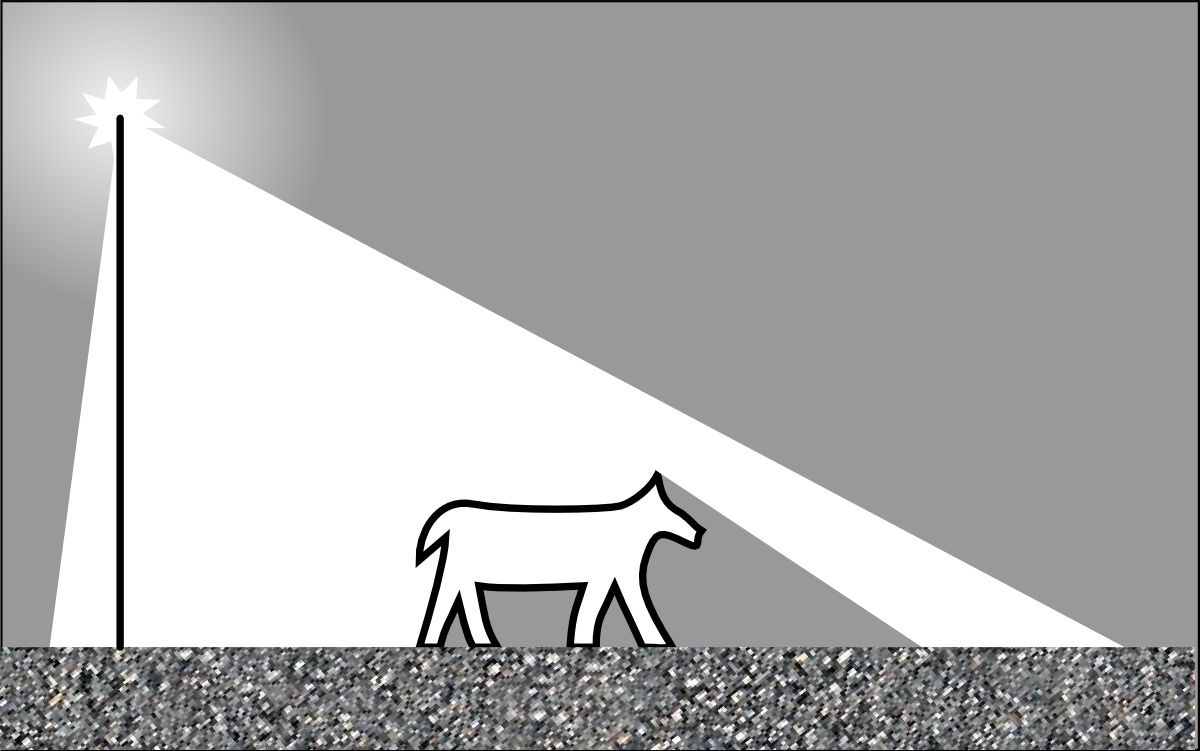
\includegraphics{04walking_dog.png}}












\problem The sides of an isosceles triangle are rotating: the lengths of 
the two (equal) sides remain fixed at 2 inch, but the angle $\theta(t)$
between them changes.




Let $A(t)$ be the area of the triangle at time $t$.  If the area increases at
a constant rate of $0.5\text{inch}^2/\text{sec}$, then how fast is the angle
increasing or decreasing when $\theta=60^\circ$?
\answer 
First, what is the area of an isosceles triangle whose sides and opening
angle you know?  This is not a formula you should memorize.  Instead try
figuring it out.  Here is the drawing:
\begin{center}
  \input ../figures/221/04problem-expandingisoscelestriangle.pdf_tex
\end{center}
The area is $\frac12 \mathsf{width}\times\mathsf{height}$, i.e.
\[
A(t)
= \mathsf{Area}
= \frac12 \times 2 \times2\sin\theta
= 2\sin\theta \; \mathsf{in}^2.
\]
This is true at all times, so we are allowed to differentiate, resulting in
\[
\frac{\dd A} {\dd t} = 2\cos \theta \frac{\dd \theta} {\dd t}.
\]
We know that $\frac{\dd A} {\dd t} = 0.5 \text{in}^2/\text{sec}$.
When $\theta=60^\circ$ we also know $\cos \theta = \frac{1} {2}$, and hence
\[
0.5 = 2\times\frac{1} {2} \times \frac{\dd \theta} {\dd t}
\text{ and thus }
\frac{\dd \theta} {\dd t} = 0.5 \mathsf{rad}/\mathsf{sec}.
\]
\endanswer




\problem A point $P$ is moving in the first quadrant of the plane.  Its motion 
is parallel to the $x$-axis; its distance to the $x$-axis is always 10 (feet).
Its velocity is 3 feet per second to the left.  We write $\theta$ for the
angle between the positive $x$-axis and the line segment from the origin to
$P$.
\answer 
The drawing:
\begin{center}
\input ../figures/221/04problem-movingpoint.pdf_tex  
\end{center}
If $x(t)$ is the $x$ coordinate of the point $P$, then
$\DS \frac{10} {x} = \tan \theta(t)$, or,
\[
10 = x\cdot \tan \theta.
\]
This is true at all times, so we may differentiate both sides
of the equation, resulting in
\[
0 = x \frac{1} {\cos^2\theta}\frac{\dd\theta} {\dd t} + \frac{\dd x} {\dd t}\tan \theta.
\]
When $\theta=\pi/3$ we have $\tan\theta = \sqrt{3}$ so $x=10/\sqrt{3}{\rm ft}$.
We are also given that $\frac{\dd x} {\dd t} = -3 {\rm ft}/{\rm sec}$
(note the minus, which
is there because the point $P$ is moving to the \emph{left}).
When $\theta=\pi/3$ we also have $\cos \theta = \frac12$.
We are led to the following equation
\[
0 = \frac{10} {\sqrt{3}} \frac{1} {(\frac12)^2} \frac{\dd \theta} {\dd t}
+ (-3) \sqrt{3},
\]
which implies
\[
 \frac{\dd \theta} {\dd t}
= 3\sqrt{3} \frac{\sqrt{3}} {10} \frac{1} {4}
= \frac{9} {40} {\rm rad}/{\rm sec}.
\]








\endanswer
\subprob  Make a drawing of the point $P$.




\subprob  Where is the point when $\theta=\pi/3$?




\subprob  Compute the rate of change of the angle $\theta$ at the moment
that $\theta=\frac\pi3$.












\problem The point $Q$ is moving on the line $y=x$ with velocity 3 m$/$sec. 
Find the rate of change of the following quantities at the moment in which
$Q$ is at the point $(1,1)$:




\subprob the distance from $Q$ to the origin,




\subprob the distance from $Q$ to the point $(2,0)$,




\subprob the angle $\angle ORQ$ where $R$ is the point $(2,0)$.








\problem A point $P$ is sliding on the parabola with equation $y=x^2$.  Its 
$x$-coordinate is increasing at a constant rate of 2 feet$/$minute.




Find the rate of change of the following quantities at the moment that
$P$ is at $(3, 9)$:




\subprob the distance from $P$ to the origin,




\subprob the area of the rectangle whose lower left corner is the origin
and whose upper right corner is $P$,




\subprob the slope of the tangent to the parabola at $P$,




\subprob the angle $\angle OPQ$ where $Q$ is the point $(0, 3)$ and $O$ is the origin $(0,0)$.




\problem \subprob The kinetic energy of a moving object with mass $m$ and velocity $v$ is $K=\frac{1}{2}mv^2$. 
If an object of mass $m=5$ grams is accelerating at a rate of $9.8$
$\textrm{m}/{\textrm{sec}^2}$, how fast is the kinetic energy increasing when
the speed is $30$ $\textrm{m}/\textrm{sec}$?




\subprob The sum of all the forces acting on the moving object is, according to
Newton, $F=ma$, where $a = \frac{dv}{dt}$.  Show that the rate at which the
kinetic energy $K$ of the object is changing is
\[
  \frac{dK}{dt} = F v.
\]




%\problem {\it Coulomb's law} states that the energy ($E$) of the interaction 
%between two ions is directly proportional to the product of the charges of two
%ions ($Q_1$ and $Q_2$) and inversely proportional to the distance ($d$) between
%their nuclei. Consider two ions of salt with charges $1+$ and $1-$. If the
%distance between the two ions is changing at a rate of $2$ pm/s, how fast is the
%energy of interaction changing when $d=165$ pm?


% The above problem has about ten errors in it: Coulomb's law is about forces and the constant of proportionality is not given, charges have units, salt is not an ion, and picometers are not defined.




\problem  Here are three versions of the same problem: 
\begin{trivlist}
\item   During a chemotherapy treatment, a tumor of spherical shape
  decreases in size at a rate proportional to its surface area. Show that
  the tumor's radius decreases at a constant rate.




\item  Helium is released from a spherical balloon so that its volume
  decreases at a rate proportional to the balloon's surface area.  Show
  that the radius of the balloon decreases at a constant rate.




\item  A spherical snowball melts at a rate proportional to its
  surface area. Show that its radius decreases at a constant rate.
\end{trivlist}




\problem Suppose that we have two resistors connected in parallel with 
resistances $R_1$ and $R_2$ measured in ohms ($\Omega$).  The total
resistance, $R$, is then given by:
\[
  \frac{1}{R}=\frac{1}{R_1}+\frac{1}{R_2}.
\]
  Suppose that $R_1$ is increasing at a rate of $0.3 \Omega/\text{min}$ and $R_2$
  is decreasing at a rate of $0.5 \Omega/\text{min}$.  At what rate is $R$
changing when $R_1=80 \Omega$ and $R_2=100 \Omega$?








\problem A runner sprints around a circular track of radius $100$ meters at 
a constant speed of $7$ m/s. The runner's friend is standing at a distance
$130$ meters from the center of the track. How fast is the distance between
two friends changing when the distance between them is $130$ meters?












\problem Ship $A$ is $50$ miles north of ship $B$ and is sailing due south 
at a constant speed of $25$ mph. Ship $B$ is sailing due east at a constant speed of $20$ mph. At what rate is the
distance between the ships changing after one hour? Is the distance
increasing or decreasing?












\problem A conical water tank with vertex down has a radius of $12$ ft at 
the top and is $30$ ft high. If water flows out of the tank at a rate of
  $14$ $\text{ft}^3/\text{min}$, how fast is the depth of the water decreasing when the
water is $20$ ft deep?












\problem A train, starting at noon, travels east at $50$ mph, while another 
train leaves an hour later from the same point, traveling north at $90$ mph. How
fast are the trains moving apart at $3$ pm?












\problem The radius of a right circular cylinder is increasing at a rate of $3$ 
in/min and the height is decreasing at a rate of $5$ in/min. At what rate is the
volume changing when the radius is $10$ in and the height is $15$ in? Is the
volume increasing of decreasing?












\problem A hemispherical bowl of radius $10$ cm contains water to a depth of $h$ 
cm. Find the radius $r$ of the surface of the water as a function of $h$. The
water level drops at a rate of $0.1$ cm/hour. At what rate is the radius of
water decreasing when the depth is $5$ cm?

\problem A cylindrical swimming pool (whose center axis is vertical) is being 
filled from a fire hose at rate of $5$ cubic feet per second.  If the pool is
$40$ feet across, how fast is the water level increasing when the pool is one
third full?


\problem Consider a clock whose minute hand is $5$ cm long and whose hour hand 
is $4$ cm long.

\subprob Find the rate of change of the angle between the minute hand and hour
hand when it is $3:00$ o'clock.

\subprob Find the rate of change of the distance between the hands when it is
$3:00$ o'clock.




\problem A baseball diamond has the shape of a square, and each side is $80$ 
feet long. A player is running from second to third base, and he is $60$ feet
from reaching third. He is running at a speed of $28$ feet per second. At what
rate is the player's distance from home plate decreasing?




\problem Doppler radar measures the rate of change of the distance from an 
object to the observer. A police officer $10$ meters from a straight road points
a radar gun at a car traveling along the road, $20$ meters away, and measures a
  speed of $30 \text{m}/\text{sec}$. What is the car's actual speed?
\answer 
The situation is thus:
\begin{center}
  \input ../figures/221/04problem-dopplerpolice.pdf_tex
\end{center}
The distance from the car to the police officer is $D(t)$.
The distance along the road from the car to the nearest point to the officer
on the road is $s(t)$.  The speed of the car (which we want to know) is $s'(t)$.
The Doppler radar measures the rate at which $D(t)$ is changing.

The relation between $D(t)$ and $s(t)$ is
\[
D^2 = s^2 + (10)^2.
\]
This is true at all times so we are allowed to differentiate the relation,
which leads to
\[
2D \frac{\dd D} {\dd t} = 2s\frac{\dd s} {\dd t}
\text{ and therefore }
\frac{\dd s} {\dd t} = \frac{D} {s} \frac{\dd D} {\dd t}.
\]
Given is that at some moment $D=20$, and $\frac{\dd D} {\dd t} = -30$
(negative because the car is moving toward the officer).
``Pythagoras'' says that $s = \sqrt{D^2-(10)^2} = \sqrt{300} = 10\surd 3$.
Therefore
\[
\frac{\dd s} {\dd t} = \frac{30} {10\surd 3} \times(-30) =
-30\surd 3\; \mathrm{m}/\mathrm{sec}.
\]

Note : the phrasing of the problem is ambiguous since ``20 feet away'' could
also be taken to mean that $s=20$ when the police officer measures the car's
speed. In that case the above computation still is valid, except at the end
one must substitute $s=20$, $D = \sqrt{(20)^2 + (10)^2} = 10\surd 5$.
This leads to
$\frac{\dd s} {\dd t} = \frac{10\surd 5} {20}\times(-30) = -15\surd 5$ m$/$sec.
\endanswer

\problem A particle $A$ moves on a circular trajectory centered at the origin 
$O$, and of radius $1$, so that the angle $\alpha$ subtended by the line segment
$OA$ and the $x$-axis changes at a constant rate $k$.  Determine the rates of
change of the $x$ and $y$ coordinates of the particle.
% This problem is unclear: the angle subtended by what?


%\problem A chemical reaction between two gas molecules occurs when the molecules 
%collide with the energy greater than an activation energy $E_a$. Assume $E_a>0$
%is constant for the given gas. The fraction of bimolecular reactions in which
%this collision energy is achieved is
%\[
%  F=e^{-\frac{E_a}{k \cdot T}}
%\]
%where $T$ is the temperature and $k>0$ is Boltzmann's constant. If the
%temperature $T$ increases at a constant rate $C$, what is the rate of change of
%the fraction $F$ of collisions that result in a successful chemical reaction?
%% This problem needs to be clarified by making explicit which quantities depend on time.


\problem A crystal in the shape of a cube dissolves in acid so that the edge of 
the cube decreases by 0.3 mm/min. How fast is the volume of the cube changing
when the edge is 5 mm?








%%\problem \groupproblem  Gas is trapped in a cylinder with a piston.  The 
%%\emph{ideal gas law} from thermodynamics says that if the cylinder is
%%not heated, and if the piston moves slowly, then one has \[ pV= C T \]
%%where $p$ is the pressure in the gas, $V$ is its volume, $T$ its
%%temperature (in degrees Kelvin) and $C$ is a constant depending on the
%%amount of gas trapped in the cylinder.
%%
%%\subprob If the pressure is 10psi (pounds per square inch), if the volume
%%is $25 \text{inch}^3$, and if the piston is moving so that the gas volume is
%%expanding at a rate of $2\text{inch}^3$ per minute, then what is the rate of
%%change of the pressure?
%%
%%\subprob The ideal gas law turns out to be only approximately true.  A
%%more accurate description of gases is given by \emph{van der Waals'
%%  equation of state}, which says that
%%\[
%%\bigl(p+\frac a{V^2}\bigr)(V-b) = C
%%\]
%%where $a, b, C$ are constants depending on the temperature and the amount
%%and type of gas in the cylinder.
%%
%%Suppose that the cylinder contains fictitious gas for which one has $a=12$
%%and $b=3$.  Suppose that at some moment the volume of gas is
%%$12\text{in}^3$, the pressure is $25$psi and suppose the gas is expanding
%%at 2 inch$^3$ per minute.  Then how fast is the pressure changing?
%%
\end{multicols}
\noproblemfont

